\documentclass[11pt]{report}
\usepackage{amsmath} %Never write a paper without using amsmath for its many new commands
\usepackage{amssymb} %Some extra symbols
\usepackage{makeidx} %If you want to generate an index, automatically
\usepackage{graphicx} %If you want to include postscript graphics
%\usepackage{mystyle} %Create your own file, mystyle.sty where you put all your own \newcommand statements, for example.
\usepackage{fancyhdr}
\usepackage{makeidx}
\usepackage{setspace}
\doublespacing
% or:
%\onehalfspacing
\makeindex

%This is for block quotes that look cool
\usepackage{ifxetex}
\usepackage[svgnames]{xcolor}
\ifxetex{%
  \usepackage{fontspec}
  \setmainfont{Linux Libertine O} % or any font on your system
  \newfontfamily\quotefont[Ligatures=TeX]{Linux Libertine O} % or any font on your system
\else
  \usepackage[utf8]{inputenc}
  \usepackage[T1]{fontenc}
  \usepackage{libertine} % or any other font package (or none)
  \newcommand*\quotefont{\fontfamily{fxl}} % selects Libertine for quote font
\fi
\usepackage{tikz}
\usepackage{framed}
% Make commands for the quotes
\newcommand*{\openquote}{\tikz[remember picture,overlay,xshift=-15pt,yshift=-10pt]
     \node (OQ) {\quotefont\fontsize{60}{60}\selectfont``};\kern0pt}
\newcommand*{\closequote}{\tikz[remember picture,overlay,xshift=15pt,yshift=10pt]
     \node (CQ) {\quotefont\fontsize{60}{60}\selectfont''};}
% select a colour for the shading
\definecolor{shadecolor}{named}{White}
% wrap everything in its own environment
\newenvironment{shadequote}%
{\begin{snugshade}\begin{quote}\openquote}
{\hfill\closequote\end{quote}\end{snugshade}}
%END


%\bibliographystyle{apsrevlong}
\bibliographystyle{plain}

%\includeonly{chaptr2} %If you just want to process chaptr2.tex

\title{Systemic Testing of Improved Bacteria Speciation Algorithms}
\author{Diego Calderon}
\date{April 2013}
\pagestyle{fancy}

\begin{document}

% To cite something use ~\cite

\pagestyle{fancy}
\maketitle

\renewcommand{\abstractname}{Acknowledgements}
\begin{abstract}
Parents \\
Cohan and Krizanc \\
TheLab \\
Thesis committee \\
Buds \\

First I would like to thank my parents for always providing their warmth and support %
when I needed it most. 
\end{abstract}
\renewcommand{\abstractname}{Abstract}
\begin{abstract}
Understanding Bacteria Speciation is difficult \\
Diversity \\
Quirkiness \\
Molecular Models for Demarcation \\
ES2 is fast \\
One line of comparison results \\
\end{abstract}
\tableofcontents

\gobbletocpage
\chapter{Introduction}
\restoretocpage

%\pagestyle{chapter}
\begin{shadequote}
The sure and definite determination (of species of bacteria) requires so much time, so much acumen of eye and judgement, so much of perseverance and patience that there is hardly anything else so \mbox{difficult}. \par--\emph{Otto F. M\"uller}
\end{shadequote}

\section{Description of Problem}
The quote above, by no mistake, graced the cover of the International Journal of Systematic and Evolutionary Microbiology for decades.
Whereas plant and animal systematists are guided by a theory-based approach to demarcating species, microbiologists have yet to agree on a set of ecological and evolutionary properties that could serve to identify bacterial species~\cite{cohan2007systematics}.
Microbiologists are naturally handicapped by the paucity of morphological differences that could aid in differentiation of closely related bacterial species.
Additionally microbiologists cannot predict which traits will cause a speciation event since bacteria are capable of receiving genes from distant relatives through a process known as horizontal gene transfer (HGT)~\cite{cohan2007systematics}.
%Thus, in order to effectively understand the microbiome we must strive towards developing a method for consistently demarcating groups, from bacterial diversity, that play distinct ecological roles~\cite{koeppel2008identifying}.
Thus, in order to effectively understand the inherent intricacy of the microbiome we must strive towards developing a method for consistently demarcating groups of bacteria that play distinct ecological roles~\cite{koeppel2008identifying}.

Initially, closely-related bacterial species were identified based on metabolic phenotype traits.
Systematists now rely on molecular approaches that utilize the decreasing cost of DNA sequencing to compare genetic information.
A 70\% cutoff was established for whole genome hybridization studies (comparing loss and gain of large segments of DNA), replaced by varying degrees of sequence identities in homologous genes~\cite{cohan2007systematics,carlo,staley1997biodiversity}.
Building on these technological breakthroughs microbiologists have taken great steps towards understanding bacteria speciation, yet they have brought into focus new difficulties.

\subsection{Diversity of Bacterial Species}
Modern molecular techniques have revealed an extraordinary diversity of microorganisms, most of which are as yet uncharacterized~\cite{bohannan2003new}.
Estimates of eukaryotic diversity fall within the range of 10 to 50 million species~\cite{may1988many}. Even though we have only observed approximately 9000 prokaryotic species, indirect approaches that do not rely on cultivation hint towards the existence of a billion or more prokaryotic species worldwide ~\cite{dykhuizen1998santa} and \textasciitilde10 million within a given habitat~\cite{gans2005computational}.
To observe biodiversity through molecular means, scientists should find organisms in highly distinct sequence clusters; since each cluster has had a long history of separate evolution they have likely evolved unique adaptations shared by the entire cluster~\cite{cohan2007systematics}.
The only rational approach to clustering such a large group of diverse organisms effectively is with a theory based molecular method that can be standardized and applied to large numbers of sequences~\cite{koeppel2008identifying}.

Current protocols for deciding bacterial lineages are functionally inadequate.
Recent ecological studies demonstrate that a named bacterial species is typically an assemblage of closely related but ecologically distinct populations~\cite{cohan2007systematics}.
Thus, within a named species established by antiquated methods, one may find distantly related organisms that do not naturally fit in with what we will define to be a cohesive species cluster, thus contradicting ideal approaches to understanding and cataloguing biodiversity.
Through such an inadequate and archaic system comprehensive study becomes impossible.

Fortunately for microbiologists organisms from every known community appear to cluster into discrete ecologically interchangeable individuals~\cite{cohan2007systematics}.
In fact, clustering is a universal feature at all levels of diversity, owning to different rates of survival and extinction~\cite{darwin1861origin}.
Our envisioned demarcation algorithm would be capable of identifying putative clusters of ecologically distinct organisms within named bacterial clades.
While accuracy is of utmost importance, due to the large numbers of potential bacterial species we would appreciate an efficient demarcation algorithm.

\begin{figure}
\centering
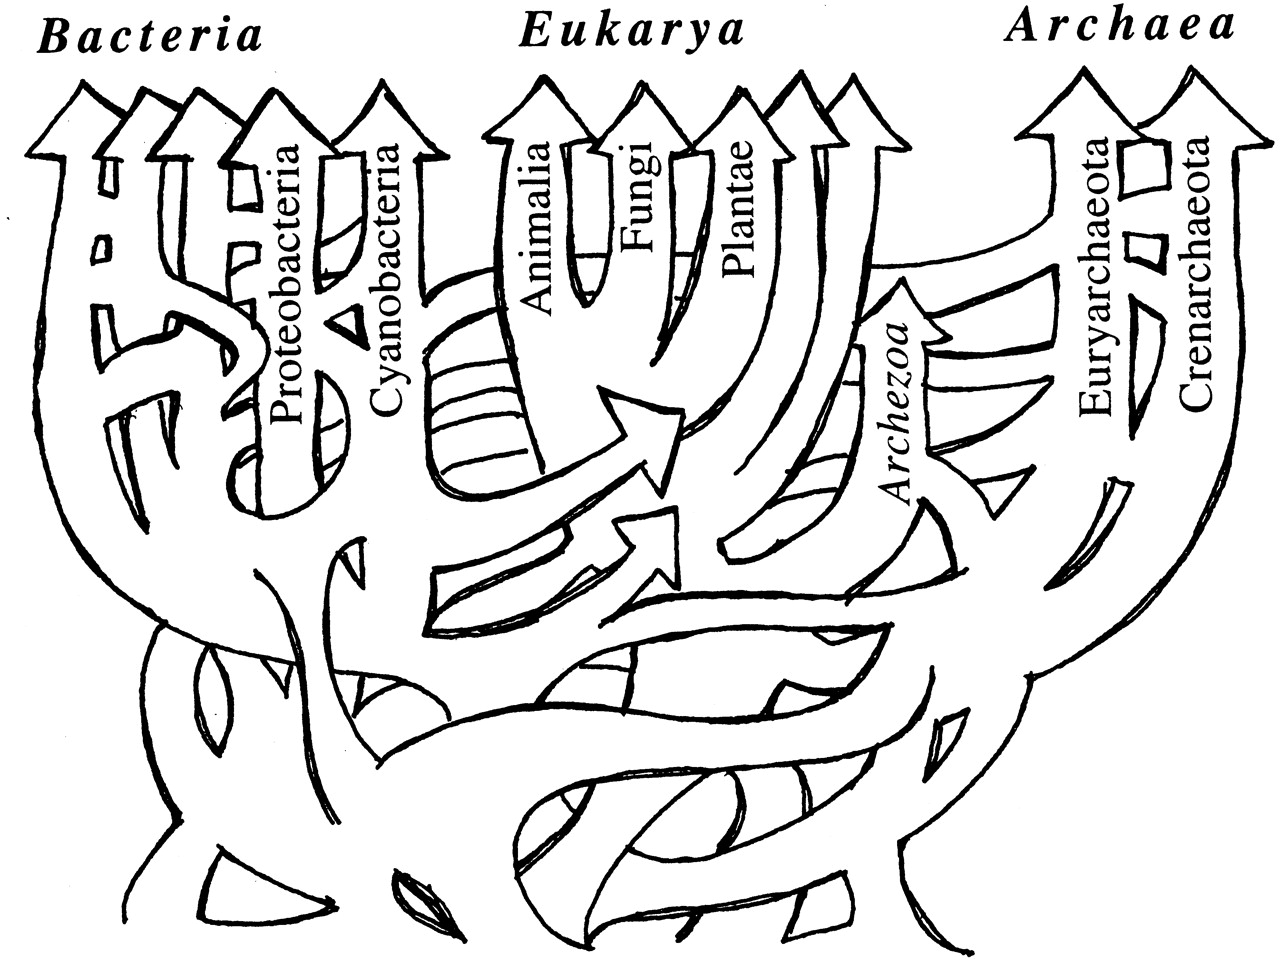
\includegraphics[scale=0.25]{images/HGTTree-CH1}
\label{fig:HGTmodel}
\caption[Model tree representing HGT.]{Model tree representing HGT. The arrows represent genetic exchange between lineages. Notice how genetic material is also shared across kingdoms. (reprinted from\protect\cite{doolittle1999phylogenetic}).}
\label{fig:HGTmodel}
\end{figure}

\subsection{Differences of Bacterial Population Dynamics}
As briefly mentioned earlier there exist peculiarities of bacterial population dynamics that complicate demarcation.
These characteristics are important to keep in mind when thinking about approaches to bacterial species demarcation.

\subsubsection*{Asexual reproduction}
Prokaryotes have the ability to reproduce clonally.
In fact, genetic exchange occurs typically through processes not tied to reproduction.
Because of low level frequencies of genetic exchange, sexual isolation is not a pre-requisite for permanent divergence between distinct ecological bacterial populations ~\cite{cohan2007systematics}.
This means that sympatric speciation becomes a common occurrence.
Early models for understanding adaptation, evolution, and speciation in these organisms often focus on clonality and periodic selection~\cite{gogarten2002prokaryotic}.
Genetic exchange plays a different role in evolution from that of plants and animals; it is assessed to be very rare and when it occurs only short segments can be successfully transferred.
Also, mutations in haploid bacteria will immediately be phenotypically expressed, resulting in rapid displacement of a parental genotype~\cite{staley1997biodiversity}, changing the dynamics of speciation.

\subsubsection*{Horizontal Gene Transfer (HGT)}
When genetic exchange does occur, in contrast to eukaryotes, bacterial genetic features can be transferred among distantly related bacteria via various genetic exchange mechanisms such as transformation and conjugation.
Genetic features may reside in the cell, on a plasmid, or become incorporated into the bacterial chromosome~\cite{staley1997biodiversity}.
HGT even can occur between very distantly related organisms e.g., between bacteria and plants or fungi~\cite{gogarten2002prokaryotic} (see Figure~\ref{fig:HGTmodel} on page~\pageref{fig:HGTmodel}).
It leads to genomes whose constituent genes have different evolutionary histories~\cite{gogarten2002prokaryotic} and can thus complicate the species identification process.


\section{Available Demarcation Software}
Today there are several freely distributed demarcation programs available: Ecotype Simulation (ES1), BAPS, GMYC, AdaptML, and newly introduced Ecotype Simulation 2 (ES2), which is an improvement on ES1.
Each is an attempt to define species as a fundamental unit, usable in practical applications a few of which I will highlight in the following section.
They all differ in background theory, resulting in different demarcations.
I will focus specifically on ES1 and the improvements resulting in ES2 which are both ecotype-based systematics proposed for identifying ecotypes, the fundamental units of bacterial ecology and evolution.
Ecotypes are ecologically distinct from each other, and each has homogenous membership~\cite{cohan2007systematics}.
More details about ecotypes will be in following chapters.

Most people are interested in direct practical applications.
Programming simulation software and bacterial speciation software, one often tends to forget about real-world applications.
The benefits of working somewhere that has a wet-lab component is that it allows researchers to focus on the theoretical and applied.

\section{Practical Applications}
We must first be able to identify the basic units operating within the system in order to understand the microbiome.
Once we have established the atomic functional unit we can then start building collections of relationships between these units.
With an understanding of microbial population dynamics comes positive real world applications.

\subsubsection*{Anticipation of future human pathogens}
Preparing for future epidemics, we should try and discover all long-standing ecotype diversity within each named pathogenic species, allowing us to anticipate disease-causing properties of each ecotype~\cite{cohan2007systematics}.
There is a large and diverse microbiome within every living organism's gut.
Many believe that certain diseases are caused by imbalances in normal microbial fauna~\cite{ballal2011host}.
We are not far from the day where we could analyze an individual's gut ecosystem and predict afflictions~\cite{ballal2011host}.

\subsubsection*{Biotechnology}
After discovering a strain with a valuable enzyme, one could then search for homologs in each ecotype closely related to the strain, potentially allowing discovery of similar enzymes with different substrates or with optima at different conditions~\cite{cohan2007systematics}.
This is particularly a useful concept for developing improved biofuel producing bacteria.
Microbial fuel cells hold great promise as a sustainable biotechnological solution to future energy needs, however current efforts to improve the efficiency of such fuel cells are limited by the lack of knowledge about the microbial ecology of these ecosystems~\cite{rabaey2004biofuel}.
Demarcation algorithms help research microbial systems, eventually uncovering beneficial pathways that the biotechnology industry can take advantage of.
However, more knowledge is necessary.
Improved biocatalysts and cellulase preparations are the major technical roadblocks to building a successful bioethanol industry~\cite{dien2003bacteria}.
Improvements in bacterial speciation understanding could save billions of dollars by uncovering more efficient ways of producing biofuels.

\subsubsection*{Simplify the burden of industrial testing of bacterial strains for their safety and efficacy in agricultural applications}
For any named species that is heterogeneous for characteristics of safety concern (such as secreted metabolites and persistence in the environment) the European Union requires that any new strain developed for release be tested for these characteristics of concern.
However, individual strains from a species known to be homogeneous for these features need not be tested, thus demarcating taxa as ecologically homogeneous units would obviate or at least lessen the burden of these tests~\cite{cohan2007systematics}.
Dealing with microbial strains can be difficult and costly, however utilizing a theory-based demarcation algorithm for bacterial identification and comparison could reduce those costs as is generally the case through standardization.

\subsubsection*{Bioremediation}
Bioremediation has the potential to restore contaminated environments inexpensively yet effectively, but a lack of information regarding the factors controlling growth and metabolism of microorganisms in polluted environments regularly limits its implementation~\cite{lovley2003cleaning}.
Demarcation algorithms could be an invaluable step in the search for microbial bioremediation tools.
If we find a gene with a positive property in one ecotype, using a theory-based speciation concept, we could quantitatively look for similar ecotypes, hypothesizing the availability of similar genes~\cite{cohan2007systematics}.
Combining models that can predict the activity of microorganisms that are involved in bioremediation with existing geochemical and hydrological models should transform bioremediation from a largely experimental practice into an industry standard program~\cite{lovley2003cleaning}.
Once again, much positive change could be brought about through the intelligent use of microbe interactions.

\subsubsection*{True quantification of ecological diversity within a community}
In the more theoretical realm, microbial ecologists are often interested in the factors that regulate community diversity across temporal and spatial scales, the impact of human activities on this diversity, and the consequences of this diversity for ecosystem processes~\cite{bohannan2003new}.
Identifying taxa at the level of ecotypes, systematics will allow microbiologists to optimize their choice of sequencing targets, because from a sample one can determine how representative it is of the environment~\cite{bohannan2003new}.
This would allow researches to gain a more comprehensive perception regarding the larger microbial ecosystem for each habitat.
%More easily giving us an idea of a microbial ecosystems species content.
%Ideally, one should choose organisms from different ecotypes to get a fuller gene content survey of the ecosystem~\cite{cohan2007systematics}.
As mentioned briefly before, current methods for surveying diversity involves binning and assigning an operational taxonomic unit without a theoretical justification.

Ecotype demarcation will allow quantification of the ecological diversity within a community, a step toward understanding the plethora of ecological interactions within natural microbial communities~\cite{cohan2007systematics}.
Such information would provide researchers and industries more accurate and objective knowledge regarding the speciation of fundamental bacterial units, towards understanding complex microbial ecosystem's intrinsic value.


\section{Outline}
%My aims for this project are several.
I have many goals for this project, of which the final result should be a production-ready version of the optimized Ecotype Simulation (ES2) software.
However, first we plan on carrying out several tests to confirm whether ES2 is accurate, and efficient in demarcating bacterial species.
I will run ES2 through the same test parameters the Cohan lab used to test ES1 against all available demarcation algorithms~\cite{carlo}; including generated datasets and environment collected sequences.
%It is important to demonstrate similar accuracy scores of ES2 to ES1.
We hypothesize that the new, more efficient, demarcating algorithm within ES2 will not significantly affect the accuracy of our output.
%Next, I want to identify the new reasonable upper limit for input size (i.e., number of sequences) for ES2.
Then I will run ES2 in conjunction with other available demarcation programs (BAPS, GMYC, AdaptML) on large generated datasets and evaluate demarcation accuracy and speed.

Chapter 1 introduced the problem that ES tries to address, and the benefits that understanding bacterial speciation will achieve.
The following chapter will go over several molecular models for bacteria speciation, their underlying algorithms, and their design and implementation in ES.
The next section discusses our approach to ES optimization and differences in ES2.
Chapter 4 will compare results of the various programs regarding demarcation accuracy and speed.
Finally, the conclusion will contain a discussion of the entire project, a section about work on future improvements, and concluding remarks.


\chapter{Prior Work}

%\begin{shadequote}
%If I have seen further it is by standing on the shoulders of giants.\par\emph{Isaac Newton}
%\end{shadequote}

%cut out up to we?
\begin{shadequote}
%Bernard of Chartres used to say that
We are like dwarfs on the shoulders of giants, so that we can see more than they, and things at a greater distance, not by virtue of any sharpness of sight on our part, or any physical distinction, but because we are carried high and raised up by their giant size.\par--\emph{John of Salisbury}
\end{shadequote}

\section{Background and Theory}
While the previous chapter succinctly summed up the purpose and motivation of developing a theory based approach to understand bacterial speciation, this chapter will provide the reader with the prerequisite knowledge necessary to thoroughly understand ES, the improvements described in chapter three, and my experimental designs in chapter four.

\subsection*{Ecotype Model of Bacterial Species}
An ecotype is defined as a bacterial cluster with individuals that are ecologically similar to one another, so much so that genetic diversity within the ecotype is limited by a cohesive force, either periodic selection or genetic drift, or both~\cite{cohan2007systematics}.
By linking species and ecological niche we take advantage of the natural clustering of organisms according to environmental resources.
Since these clusters are evolving together we do not need to utilize morphological differences and can instead use a molecular approach for demarcation.

Ecotypes have all the dynamic properties of a species, each is a cohesive group, different ecotypes are irreversibly separate because they are out of range of one another's cohesive force, and because recombination is too rare to prevent their adaptive divergence; they are by definition ecologically distinct, which allows them to coexist into the future~\cite{cohan2007systematics}.
Or, essentially the fundamental unit of microbial ecosystems.
Efforts to define prokaryotic species according to these properties have differed most profoundly in the forces of cohesion thought to be most important for prokaryotic species~\cite{cohan2008origins}.
ES uses one model in particular to understand ecotype bacterial speciation.

\subsection*{Stable Ecotype model}

\begin{figure}[h!]
% \caption{Three classes of mutation and recombination events that determine ecotype diversity in bacteria. Circles represent different genotypes, and asterisks adaptive mutations. (A) Periodic selection purges diversity. (B) Ecotype formation creates diversity. (C) Extinction events SHOULD I CUT THIS OUT?.(reprinted from \protect\cite{cohan2007systematics})}
 \centering
 \label{fig:StableEvents}
 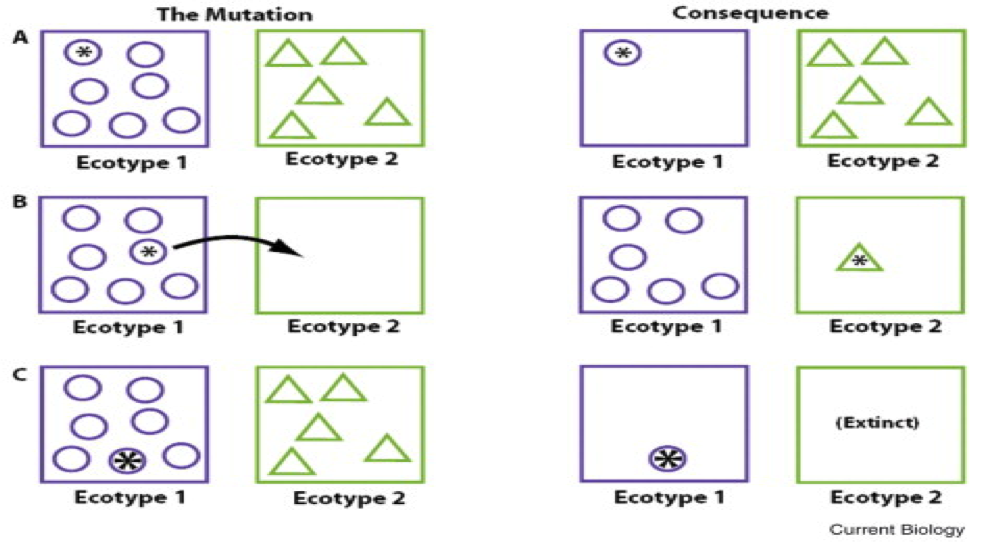
\includegraphics{images/StableEcotypeEvents-CH2}
 \caption[Events predicted by the Stable Ecotype model.]{Three classes of mutation and recombination events that determine ecotype diversity in bacteria. Circles represent different genotypes, and asterisks adaptive mutations. (A) Periodic selection purges diversity. (B) Ecotype formation creates diversity. (C) Extinction events (reprinted from \protect\cite{cohan2007systematics}).}
 \label{fig:StableEvents}
\end{figure}

In the Stable Ecotype model, ecotypes are created and extinguished at a very low rate, and during its long lifetime an ecotype is recurrently purged of its diversity by periodic selection events~\cite{cohan2007systematics}.
Ecotypes are formed rarely enough so that they can accumulate its own set of unique mutations while diversity is purged, yielding a correspondence between ecotypes and sequence clusters for any gene shared among ecotypes~\cite{cohan2008origins}.
This fact, hinted at earlier, is what allows ES to identify separate ecotypes based on environmental function without knowledge of particular phenotypic mutations.
Diversity quashing events are referred to as periodic selection events, see Figure~\ref{fig:StableEvents}a.
An individual of an ecotype acquires a mutation that improves its fitness within that ecological niche, which results in a diversity purge, due to low recombination rates in bacteria, where other organisms in the ecotype without the adaption become extinct.
Genetic drift is another event that results in diversity purges, however it is normally quite rare (except in small sample sizes).

%Describes relationship of periodic selection events and ecotype formation event
%I don't think this is correct, double check!!
Early during speciation, a new ecotype's niche may rely on proportions of resources used and may be vulnerable to extinction by periodic selection caused by an adaptive mutation within the parental ecotype.
However, a single HGT event may transfer the adaptive mutation across ecotypes, and could thereby prevent extinction of one ecotype by another~\cite{cohan2008origins}.
In this case an ecotype formation event occurs, see Figure~\ref{fig:StableEvents}b.
The ecotype-transcending adaptation allowed an ecotype speciation event to occur. In the figure an individual of an ecotype developed an adaptation that went on to colonize a new niche creating a new ecotype.

Now we have an event to account for anagenesis, or accumulation of changes over time along a single lineage, referred to as periodic selection, and cladogenesis, or irreversible splitting of lineages, referred to as ecotype formation.
To complete the dynamics of the Stable Ecotype model, extinction events are also possible, see Figure~\ref{fig:StableEvents}c.
An ecotype, obviously, can go extinct.
Previous work done in the Cohan lab was done to develop an algorithm based on the Stable Ecotype model, which eventually became known as Ecotype Simulation (ES).


\section{The Algorithm}

\begin{SCfigure}
 \caption[Phylogenetic tree representation of typical Stable Ecotype model case.]{ The Stable Ecotype model, in which ecotype formation is relatively rare, and periodic selection events (represented by asterisks, frequently purge all diversity from within each ecotype. Extinct lineages are dotted, while existing ones are solid. Time progresses from bottom to top. This model predicts a one-to-one correspondence between sequence clusters and ecotypes (reprinted from \protect\cite{cohan2008origins}). }
 \centering
 \label{fig:StableTree}
% 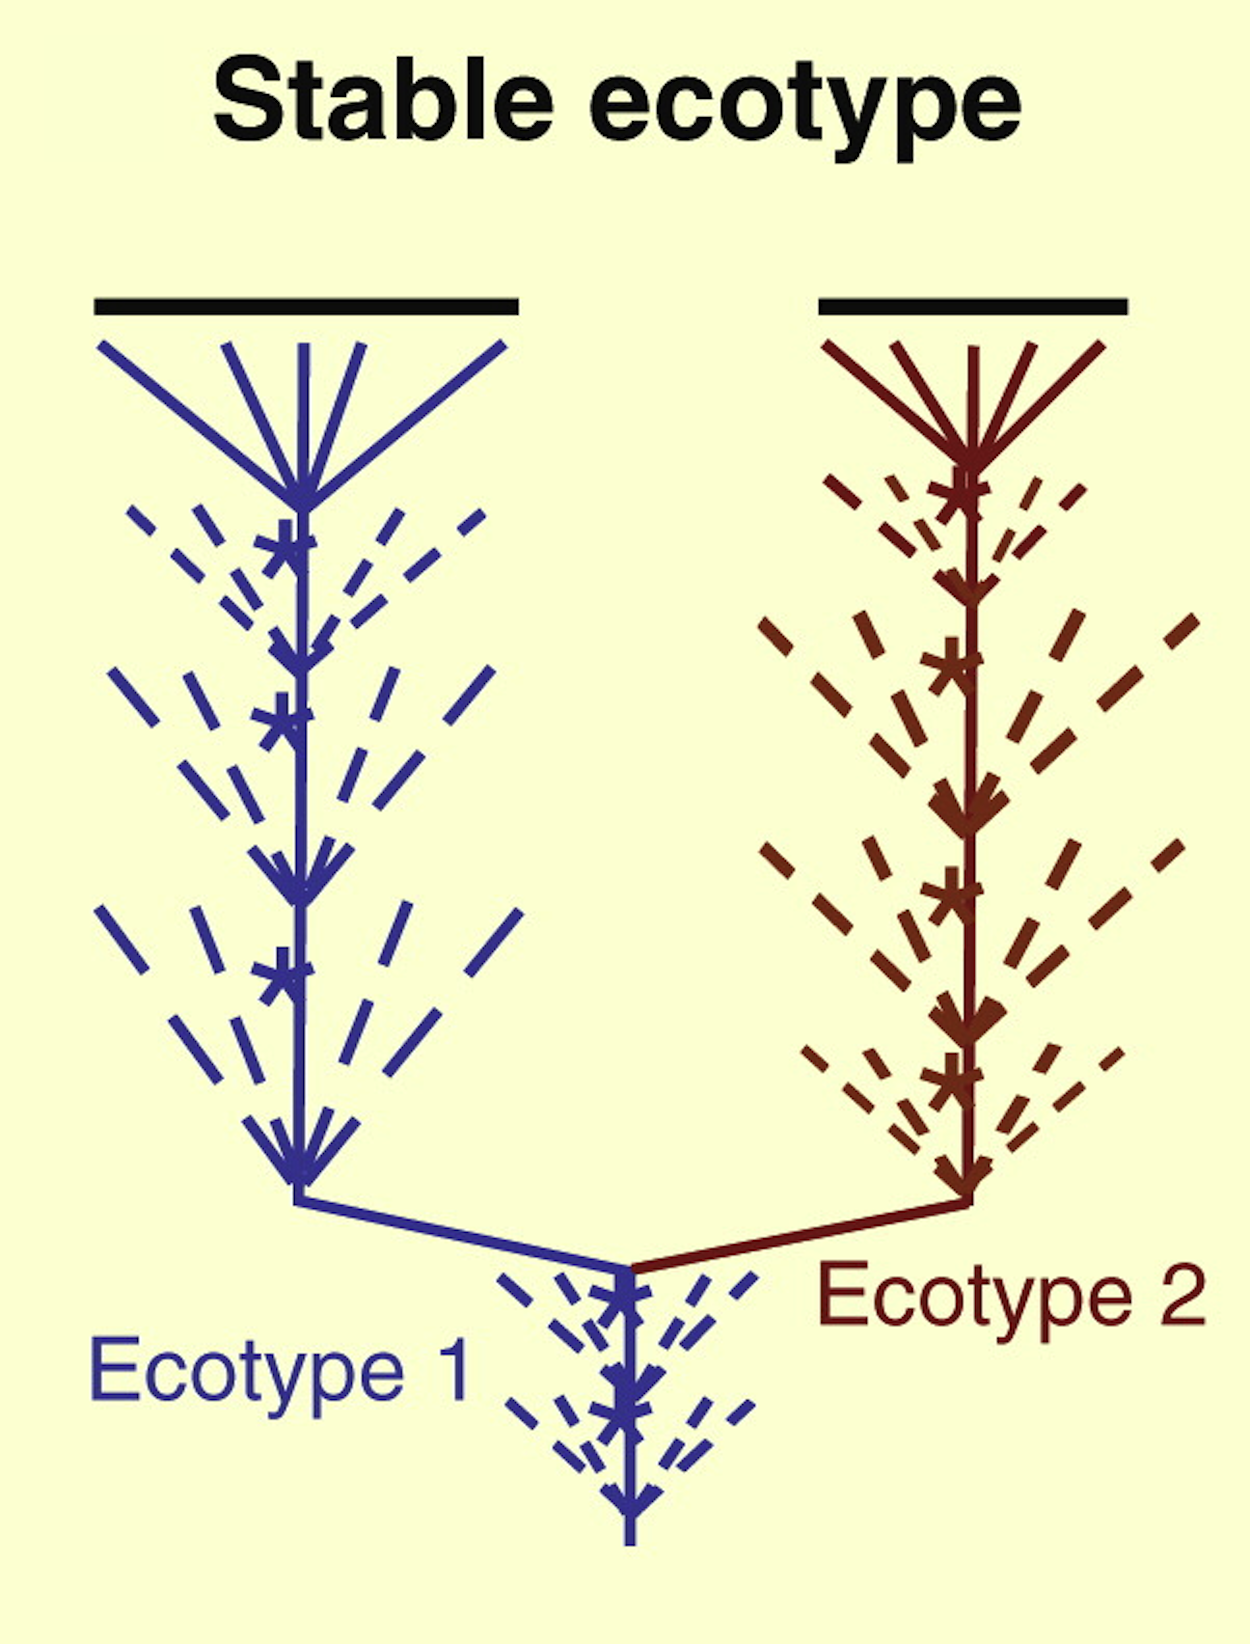
\includegraphics{images/StableTree-CH2}
 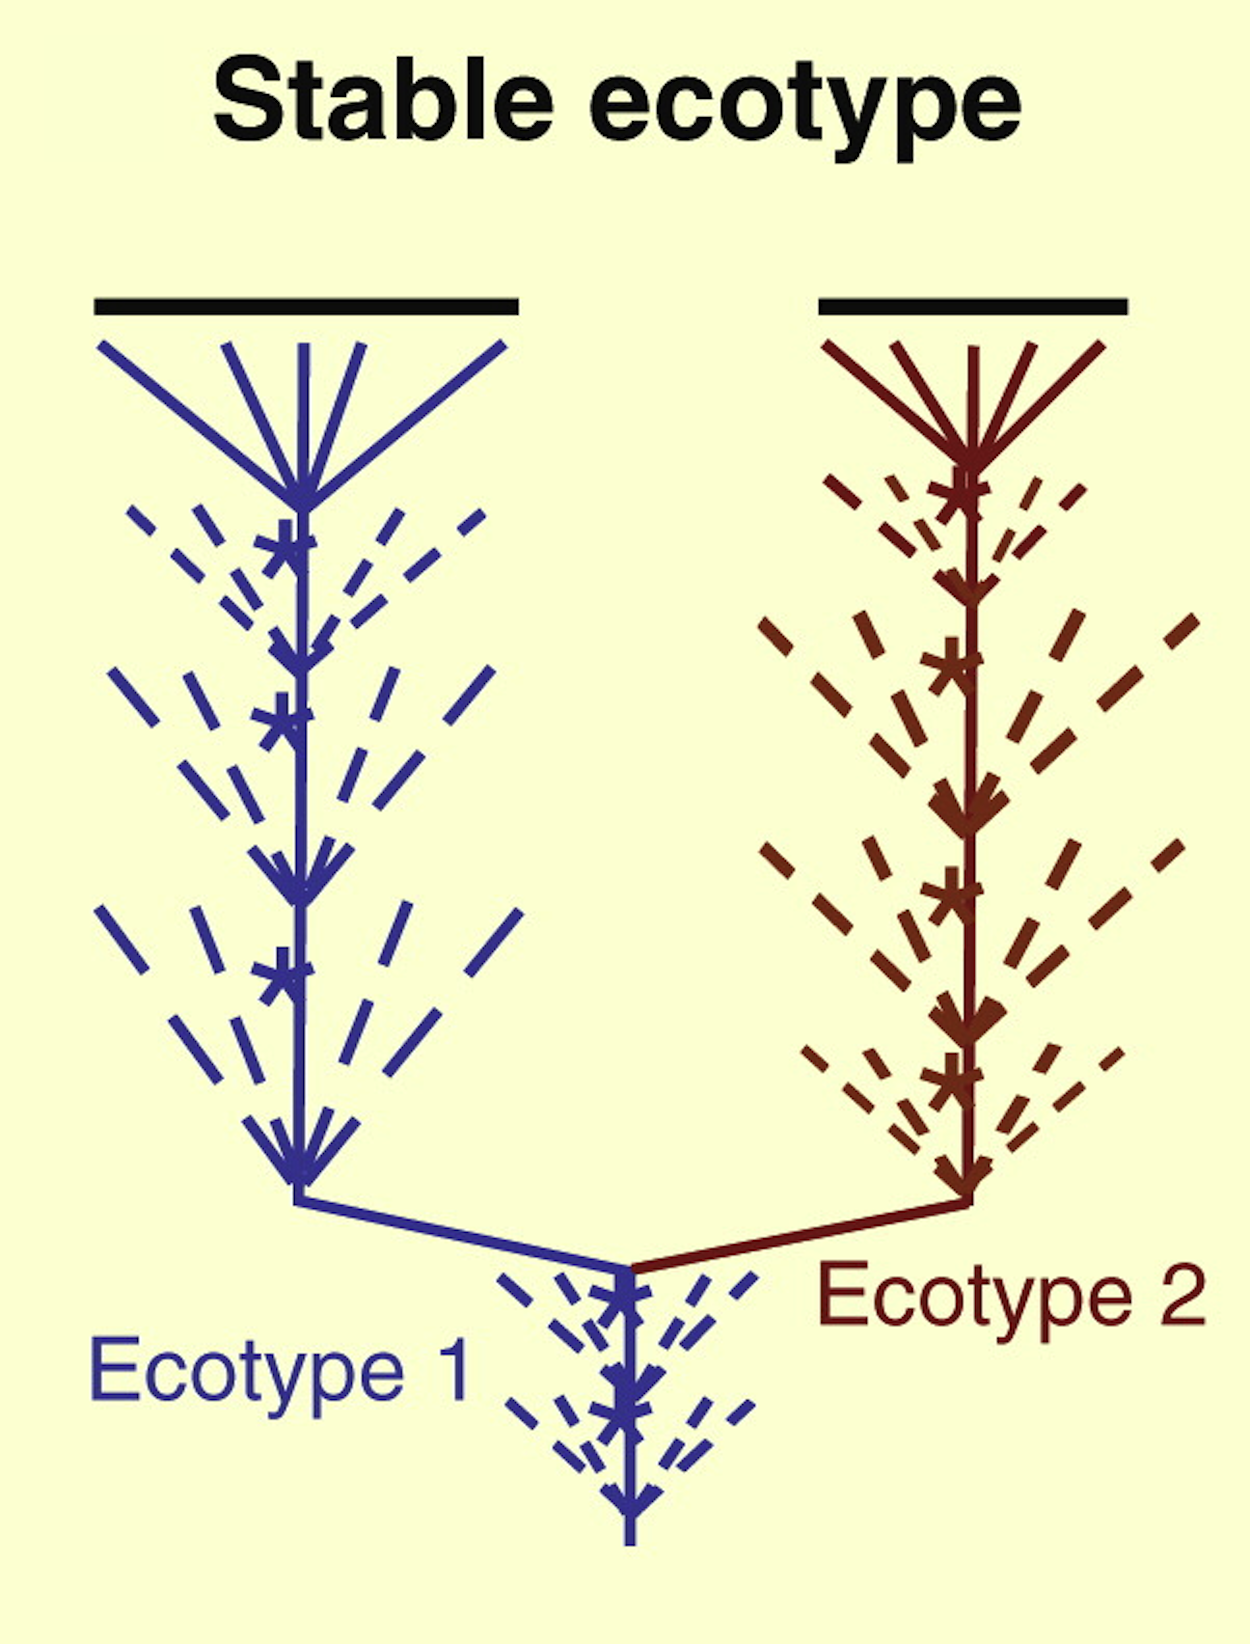
\includegraphics[width=0.5\textwidth]{images/StableTree-CH2}
 %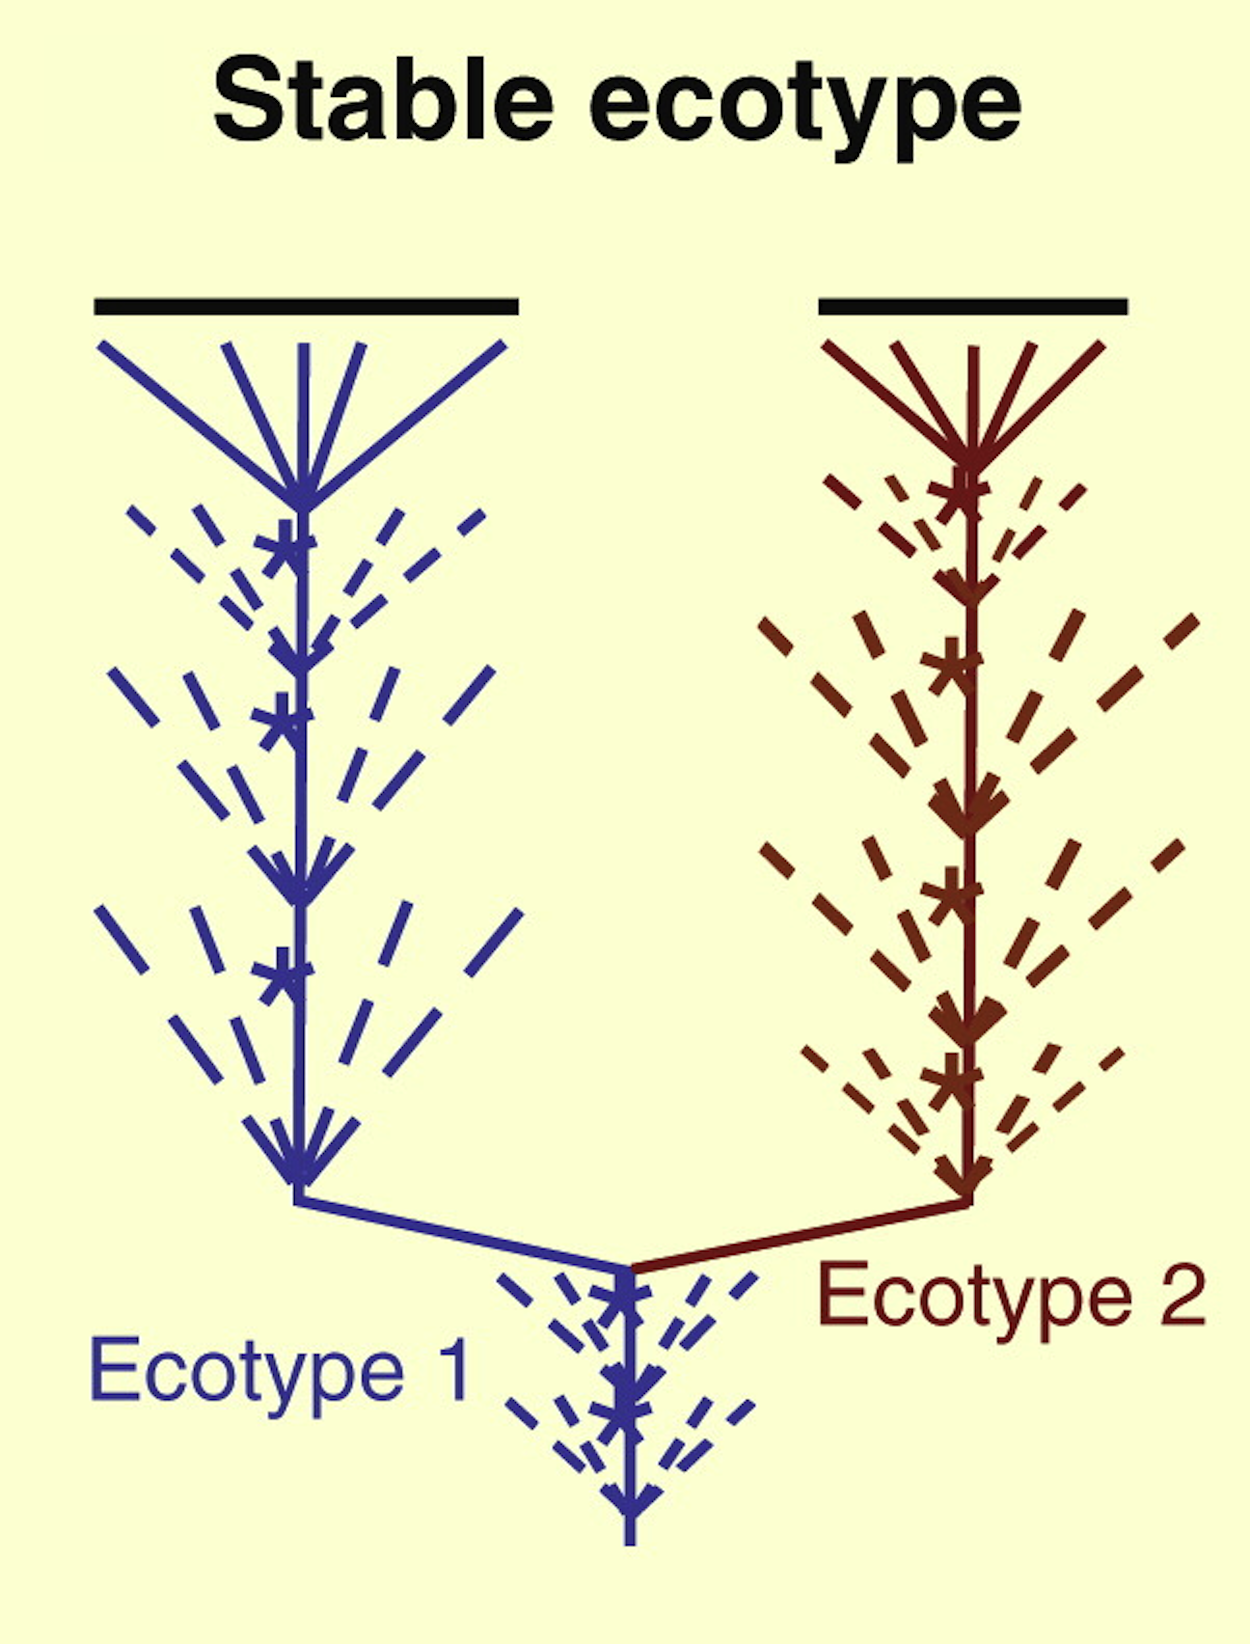
\includegraphics[scale=2.5]{images/StableTree-CH2}
\end{SCfigure}

Utilizing premises established in the Stable Ecotype model we hypothesize a phylogenetic tree similar to the one represented in Figure ~\ref{fig:StableTree}.
Here we can see that ecotype formation is relatively rare, while periodic selection (asterisks) keep the branches of the tree pruned.
At the point of divergence (where the two solid lines separate into ecotype 1 and 2), organisms from the two separate ecotypes are closely related.
However over time and through various purification events adaptive mutations accumulate.
Notice that the two clades are totally free from each other's periodic selection diversity quashing~\cite{cohan2007systematics}.
This is an important feature of separate ecotypes, because we can later observe the differences acquired from separate evolutionary histories.

Theory and empirical evidence hints that these boundaries correlate to ecological niche~\cite{cohan2007systematics, cohan2006sequence, ward2006cyanobacterial, cohan2006toward}.
To identify the system's fundamental elements takes three steps.
First, observe the communities evolutionary history.
Second, simulate evolutionary history as hypotheses of various descriptive parameters, resulting in a most likely parametric characterization of observed history.
Finally, demarcate individuals into ecotypes.

\subsection*{Observing evolutionary history}
Since the clades are evolving independently we can use the molecular clock characteristic of specific ubiquitous genes.
The gene we choose to measure between organisms must be present throughout.
For this reason ES typically takes in ribosomal gene 16s, chaperone dnaJ, or gyrase subunit gyrA sequences  as input. Most living organisms have closely related homologues.

From genes we can build a phylogeny that predicts a likely evolutionary history, simply based on sequence distances.
Because, ES only analyzes sequences from non-extinct organisms, the Stable Ecotype model predicts that lineage divergence will be low.
And the bacterial diversity sampled is going through various stages of periodic selection purification, thus the end of the phylogeny (temporally closest to the present) will appear frayed.

\subsection*{Simulating evolutionary history}
Starting from observed sequences as separate clusters, ES simulates common divergence, and cohesion events backwards in time, which reduce the number of groups until there is only one cluster representing the closest ancestor.
From that closest ancestor representation with known gene mutation rates, we can simulate sequence diversity through time and generate a collection of gene sequences.
Now this simulated output can be compared to the observed evolutionary history to check for similarity.
By running many (approximately in the millions) simulations, ES develops a max likelihood parametric characterization of the observed phylogeny. 

\subsection*{Demarcating ecotypes}
The parametric characterization helps decide how to separate individuals into clusters.
ES progresses temporally from the root of the phylogeny towards the present, analyzing each subtree.
Once there is a certain likelihood that that subtree consists of only one ecotype the demarcation program annotates it as such.


\section{Ecotype Simulation}
%
%   SHOULD WE INCLUDE SAMPLE INPUTS AND OUTPUTS FOR EACH PROGRAM?
%
The current iteration of ES is a GNU General Public Liscenced free (as in freedom, not beer) and open source software written mainly in Fortran90 with a Java graphical user interface (GUI) that runs on most platforms.
As inputs it takes a FASTA format file that consists of aligned DNA gene sequences (usually genes mentioned earlier; concatenated if multiple), and a corresponding phylogeny, either supplied by the user as a Newick format tree or generated by an optional dependency (Phylip ~\cite{felsenstein1989phylip}) on runtime.
The implementation follows our approach discussed in the previous section, namely, observed evolutionary history analysis, simulation, and demarcation.

\subsection*{Binning}
First the input sequences go through pre-processing to remove nucleotide gaps, and correct for poly-nucleotide chain reaction (PCR) error.
Next an $O(n^2)$ space divergence matrix is created using a modified Manhattan (or taxicab) distance metric, where at each base pair position if the two sequences being compared differ in nucleotide we increase the distance by one then divide the total by half the number of base pairs in the sequence.
The divergence matrix is used to facilitate complete linkage clustering of the sequences, described by the equation $$D(X,Y)= \max_{x\in X, y\in Y} d(x,y)$$ where $d(x,y)$ is the distance between the two elements $x \in X$, and $y \in Y$, and $X$ and $Y$ are two clusters of elements.
The implementation is a naive (i.e., $O(n^3)$) and hoards a lot of space because of the divergence matrix; there is room for improvement here (I will go into clustering in detail the following chapter). 

\begin{figure}[h!]
 \centering
 \label{fig:Binning}
 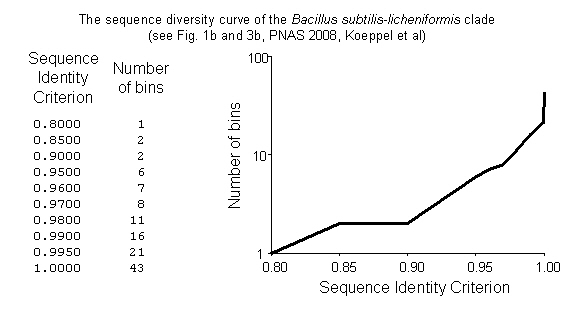
\includegraphics[scale=1.75]{images/Binning-CH2}
 \caption[Sequence identity graph and example output produced by binning.]{An example output of information from the initial binning of wild-type sequences (adapted from \protect\cite{koeppel2008identifying}). }
  \label{fig:Binning}
\end{figure}

After binning we observe a sequence identity graph as in Figure \ref{fig:Binning}.
The $x$-axis refers to percent identity between sequences and the $y$-axis the number of bins or clusters.
At low sequence identity criterions there are less bins with more sequences in each, and at $1.00$ sequence identity we have unique sequences.
A good way to visualize this sequence identity graph is as a linear representation of a phylogeny.
The slope is shallow during lower sequence identities similar to how in a tree we typically see low levels of cladogenesis.
But, as you approach the end of a tree there typically is a fraying of the tips, and in the identity graph there is a corresponding steepening of slope, see Figure \ref{fig:SpeciationGraph}. %why isn't this correct?
Concave departures from an exponential relationship indicate an overabundance of highly divergent lineages (i.e., a very genetically diverse community); convex departures indicate an overabundance of closely related lineages (i.e., a less genetically diverse community~\cite{bohannan2003new}.

We can describe the essence of this graph in four parameters: $npop$, sigma ($\sigma$), omega ($\Omega$), and drift (d), which represent the number of ecotypes, rate of periodic selection (PS), rate of ecotype formation (EF), and drift (d), respectively.
By finding close approximations of npop, $\sigma$, $\Omega$, and d we can observe ecotype boundaries within the clade that hypothetically correspond to ecological niche (as stated earlier).

\subsection*{Simulations and likelihood evaluation}
The simulation aspect of ES begins with a process of backwards simulation that stochastically (like a roll of a dice) produces a phylogenetic representation of the history of the community.
Think of a node that represents each input sequence (i.e., number of nodes equals number of input sequences) which coalesce (due to PS, EF, or D; indicated by gray circles in Figure \ref{fig:SpeciationGraph}) as ES steps backward in time.
Backwards simulation serves as a scaffold for forward simulation, which produces corresponding mutational nucleotide substitution throughout the history of the clade.

Initially a set of $v$ contemporary organisms (representing those sampled from the environment) are randomly distributed among $n$ ecotypes (in the case of Figure \ref{fig:SpeciationGraph}, $v = 14$, and $n = 3$).
Working backward from the $v$ organisms in the present, the process of EF, PS, and D occur stochastically in time according to their respective predetermined rates ($\Omega$, $\sigma$, and d).
Each event coalesce one or more lineages into  a single ancestral lineage.
The backward phase of the simulation ends when all of the branches have coalesced into a single node, which represents the most recent common ancestor of the sampled organisms.

\begin{figure}[h!]
%INCLUDE?
%Note that in the backward-looking view of the coalescence formulation, each PS appears as a coalescence event, in which all lineages after the PS coalesce into the survivor of the PS event. Likewise, each D event appears in this backward-looking view as the coalescence of a pair of lineages within an ecotype (e.g., two contemporary lineages coalesce into lineage D1 to reflect the increased representation of lineage D1 after the random loss by drift of lineage D2). 
%Because $\Omega$ is the net rate of EF events, taking into account extinction, we include in the simulation only those EF events resulting in ecotypes that survive into our contemporary sample.

  \centering
   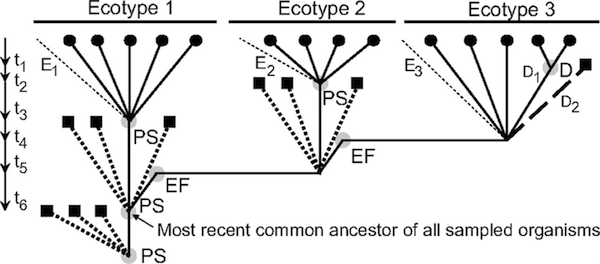
\includegraphics{images/Speciation-CH2}
   \caption[Detailed phylogeny with putative ecotype simulation events.]{A phyolgeny representation of the ecotype simulation algorithm. The algorithm simulates the evolutionary history of the organisms sampled from nature under different values for the net rate of ecotype formation (EF), rates of periodic selection (PS), drift (D), and the number of ecotypes in the sample. It only considers existing individuals (black circles) from non-extinct lineages represented by bold lines. Previously extinguished lineages, due to past PS or D events, are represented by dotted lines and squares (reprinted from \protect\cite{koeppel2008identifying}).}
   \label{fig:SpeciationGraph}
\end{figure}

Forward simulation begins when a sequence, the same length of a sample individual, is assigned to the most recent common ancestor.
As time progresses nucleotide substitutions occur stochastically between each pair of nodes (according to the time between the events determining the nodes) in the phylogeny derived from the backward simulation. 
This continues until we reach the contemporary organism nodes, resulting in a matrix of pairwise sequence divergence between $v$ contemporary organisms.

Now ES can conduct the same complete-linkage clustering analysis briefly described in the previous section to illustrate a sequence identity graph, which can be compared to the observed sequence identity graph.
If we place our simulated sequence identity graph line on top of the observed sequence identity graph, at each bin level we can see within a pre-determined factor (or precision factor) if the simulated line matches the observed line.
Success is determined by whether or not these two lines match within this factor of closeness.
If the simulation and observed graphs are too far apart, ES records the repetition as a failure.
Based on many (i.e., in the hundreds) of runs, each one evaluated for success or failure, we gather information to form a max likelihood estimation of $npop$, $\Omega$, $\sigma$, and d. However, how does one decide on variable seeds?

\subsection*{Bruteforce and Hillclimbing}
Utilizing simulations explained in the previous section ES conducts a search for high likelihoods over a multi-dimensional plane (four parameters).
To search as much of that space as possible we lay a grid of points over the landscape of likelihoods where each point is a simulation of many hundred repetitions.
By running those tests we begin to observe a rough sketch of hills and valleys of likely parameters.
The even distribution of points with a lack of insight is referred to as Bruteforce (see Figure \ref{fig:Flow}a).
Bruteforce outputs a range of parameters that should contain some local maximum likelihood.
The range of likely parameters is then passed through an optimization program known as Hillclimbing (see Figure \ref{fig:Flow}b).

Hillclimbing is  downhill-simplex or Nelder-Mead approach to optimization.
A chosen parameter solution is more thoroughly tested (i.e., with 10000 replicates), and likelihoods are calculated for the six precision values (i.e., 5x, 2x, etc.).
The program then calculates how long it would have to run to generate 50 success based on the duration of the previous step.
If too much time is required then Hillclimbing runs with a more general precision value.
I PLAN TO GO INTO MORE DEPTH ON HILLCLIMBING HERE!
%Describe exact detail of hill climbing optimization. Ask for background paper?


\begin{figure}[h!]
 \centering
 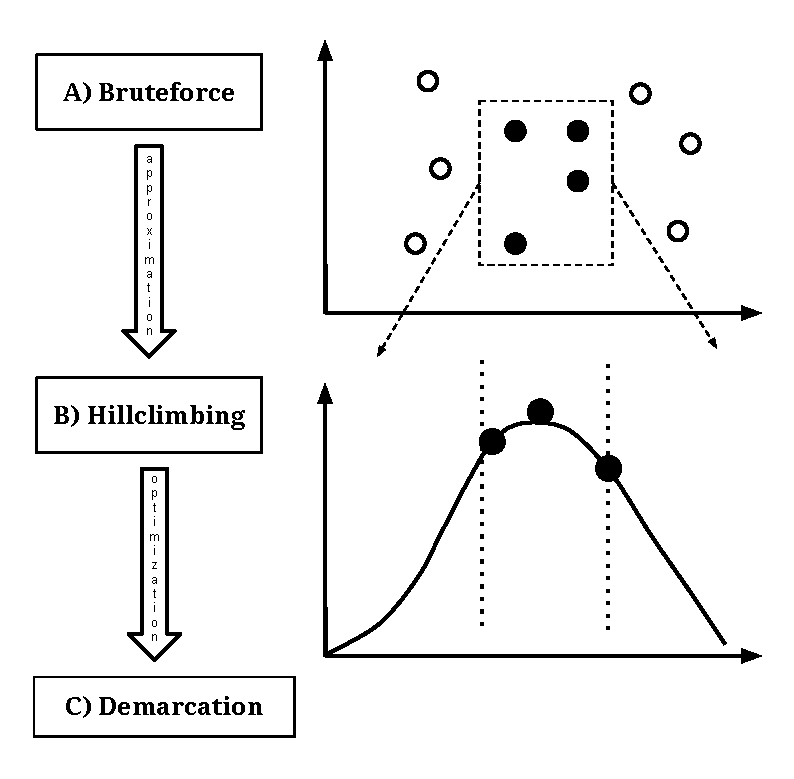
\includegraphics[scale=0.75]{images/ESFlow-CH2.pdf}
 \caption[Ecotype Simulation program flow diagram.]{This is the program call flow of ES. Circles represent simulations, filled are high likelihood successes, while empty are failures. Bruteforce distributes test parameters along the grid, and Hillclimbing figuratively climbs the likelihood hill to find local a maximum (figure created with help from Lingyuan Ke). }
 \label{fig:Flow}
\end{figure}

\subsection*{Demarcation}
With most likely estimations of $npop$, $\sigma$, $\Omega$ we proceed to Demarcation (see Figure \ref{fig:Flow}c).
Demarcation uses the phylogeny generated by the observed divergence matrix and the maximum likelihood parameters produced from Hillclimbing optimization (see Figure \ref{fig:Flow}b - c).
ES ships with a manual demarcator, however for my work we used an auto-demarcator that uses a demarcation confidence interval program.

The auto-demarcator starts at the closest common ancestor and recursively runs confidence interval tests for $npop$ on subtrees.
A confidence interval involves starting with a set of parameters as a seed, determining percent likelihood (using simulations discussed previously), and deciding whether there is a 95\% likelihood of the subtree only containing a single ecotype.
If so we identify that group of samples as a single ecotype and stop the recursive tree descent.

\section{Ecological Correlation}
Once any algorithm is developed, we must prove correctness.
In the case of ES, we want to evaluate whether or not predicted demarcations correlate to observed samples.
The Cohan group even recommend ecologically checking ES predicted ecotypes, because under various evolutionary models (other than the Stable Ecotype model), a single ecotype may contain multiple sequence clusters \cite{koeppel2008identifying, connor2010ecology}.

This is easier said than done.
Over the past four years the Cohan lab and collaborators have travelled to unique environments around the world gathering samples of bacterial ecosystems and analyzing them with demarcation programs.
Following is a short discussion of a few of these studies focused on further insights achieved with ES.

%\subsection*{Radio Facility Wash Paper}
\subsection*{Ecology of Speciation in the Genus \emph{Bacillus}}
%The ecology of speciation in Bacillus connor2010ecology
Scientists sampled bacteria from the \emph{Bacillus subtilis-Bacillus licheniformis} clade from sites differing in solar exposure and soil texture within a Death Valley canyon.
Within the sample clade they hypothesized ecotype demarcations based on DNA sequence diversity through the clade's evolutionary history analysis with ES.
Ecotypes demarcated were found to be significantly different in their associations with solar exposure and soil texture~\cite{connor2010ecology}.
In the study they were attempting to provide new protocol for describing and discovering the ecotypes of a microbial clade.
However, they were careful to show that groups predicted by ES correlate to environmental characteristics; one such significant example was the solar exposure.
Clearly connecting species and ecologically niche.

The recognized species and subspecies of the sampled clade were found to be nearly identical to the ecotypes demarcated by ES.
Nevertheless, the taxa recognized do not appear to encompass the full ecological diversity of the clade~\cite{connor2010ecology}.
ES predicted putative ecotypes not recognized by recognize species and subspecies, in one case they identified the ecological dimensions of divergence, suggesting that the \emph{B. subtilis-B. licheniformis} clade is replete with newly divergent ecotypes~\cite{connor2010ecology}.

%\subsection*{Yellowstone hot spring paper}
\subsection*{Fine-Scale Distribution Patterns of \emph{Synechococcus} Ecological Diversity in Microbial Mats of Mushroom Spring, Yellowstone National Park}
%Fine-scale distribution patterns of Synechococcus becraft2011fine
Scientists sampled the \emph{psaA} (which encodes a photosynthetic reaction center protein) locus from the genus \emph{Synechococcus} and studied distribution variants at 1$^\circ$C intervals along the effluent flow channel at 80-$\mu$m vertical-depth intervals throughout the upper photic layer of the microbial mat~\cite{becraft2011fine}.
Once again a microbial community is sampled for a common DNA sequence.
In this case the thinking is that the various layers of bacterial organisms differ in photosynthetic specialization, thus the choice of \emph{psaA}, which offers more molecular resolution.
However, since we use a molecular approach that measures a single gene carefully, even correlation between ecological niche and ecotype provides evidence for accurate demarcation.

The microbial mats at the 60 and 63$^\circ$C sites both exhibited steep gradients of O$_2$, pH, and irradience with depth, leading to microenvironmental niche opportunities in the mats.
The group used denaturing gradient gel electrophoresis (DGGE) to track the distributions of PEs predicted by ES.

%\subsection*{Death Valley Salinity}
\subsection*{Diversity of Bacteria and Archaea in hypersaline sediment from Death Valley National Park, California}
%Death Valley salinity kim2012diversity
The objective of this study was to analyze the evolutionary history of microorganisms from the domains Bacteria and Archaea in hypersaline sediment from Death Valley National Park~\cite{kim2012diversity}. 
They looked at a region of the 16s rRNA gene.
A set of 130 \emph{Bacillus} isolates formed a subclass of the \emph{B. subtilis-B. licheniformis} clade, forming four newly discovered clades (see Figure \ref{fig:DeathES}) that were each identified as an ecotype by ES. Evidence for ecological divergence among the putative ecotypes is provided by the significant tendencies of these groups to be isolated from different media~\cite{kim2012diversity}.

Here we see another example of exploring microbial diversity through molecular means.
But the list of possible applications is endless.
In fact we are at the point where increasing the input size is quite important so we can attempt to grasp a more complete picture of bacterial diversity (which as we have already established is probably in the millions~\cite{cohan2008origins}).


\begin{figure}[h!]
\centering
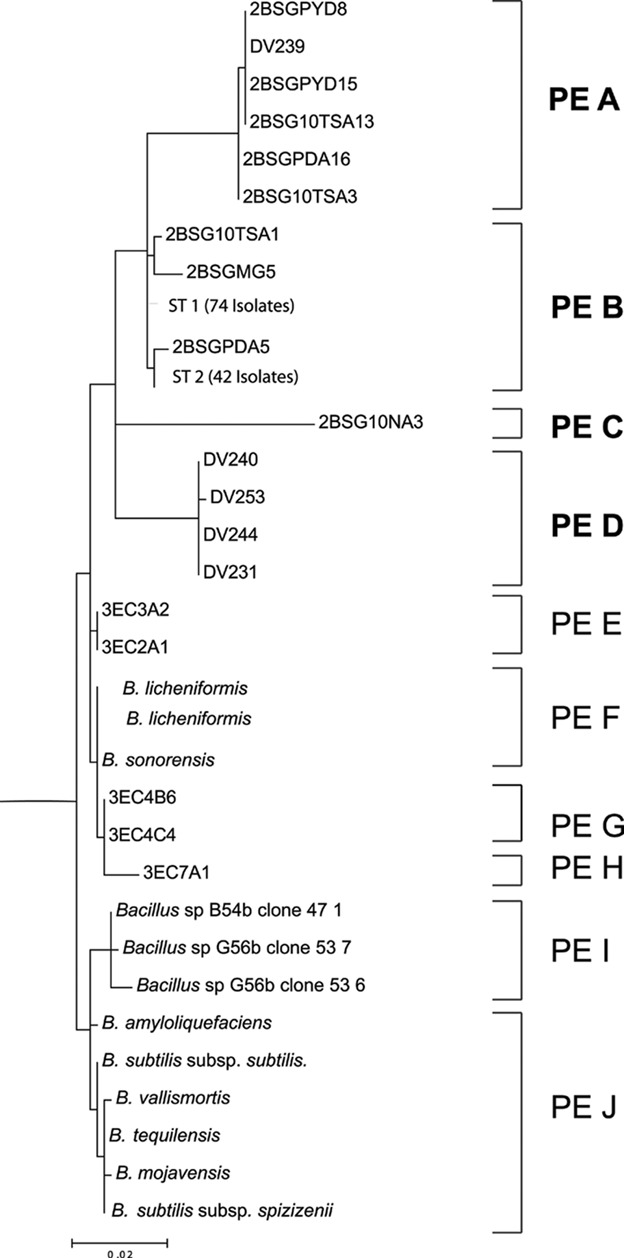
\includegraphics[scale=0.45]{images/DeathValleyES-CH2}
\caption[Example ES analysis of 16s rRNA sequences of isolates from the \emph{B. subtilis-B.licheniformis} clade.]{Maximum likelihood phylogeny and Ecotype Simulation analysis of 16S rRNA sequences of isolates from the \emph{B. subtilis-B. licheniformis} clade. All isolates of this study from this clade were members of a previously unknown subclade that Ecotype Simulation demarcated into Putative Ecotypes A-D (in bold); previously studied organisms from other environments were members of Putative Ecotypes E-J. The tree is rooted by \emph{B. halodurans} strain C-125 (reprinted from\protect\cite{kim2012diversity}).}
\label{fig:DeathES}
\end{figure}

\section{Chapter Summary}
Here we introduced the ecotype model of bacterial species, which defines species as a bacterial cluster with genetic diversity limited by a cohesive force.
Then explore various possible events affecting evolutionary history in the Stable Ecotype model of bacterial speciation, which provide the grounding in theory necessary to develop an algorithm for demarcation.
Specifically through the use of periodic selection, drift purification, and ecotype formation events.

After generally discussing the algorithm behind ES, we got our hands dirty and described each important step of ES in detail, including Binning, simulations, Bruteforce, and Hillclimbing (see Figure~\ref{fig:Flow}).
Finally, I briefly surveyed a few studies where we attempted and succeeded in displaying the statistical significance of ES bacterial species demarcation.

In the following section I will discuss the work we have done recently in improving ES.





\chapter{Improvements of Ecotype Simulation}

%\begin{shadequote}
%\begin{center}
%    \Large\begin{verbatim} 
%        Harder, Better, Faster, Stronger
% \end{verbatim}  
%\end{center}
%\par--\emph{Daft Punk}
%\end{shadequote}

\begin{shadequote}
\begin{center}
    \Large\begin{verbatim} 
             Citius, Altius, Fortius
 \end{verbatim}  
\end{center}
\par--\emph{Olympic Motto}
\end{shadequote}
%%Faster, Higher, Stronger


\section{Improvements}
ES1 set hard input size limits of 2000 sample sequences of at most 3000 nucleotides~\cite{koeppel2008identifying}.
However, I doubt it was ever run with even close to that many sequences.
When run on input sizes of greater than only one hundred sequences time became a limiting factor.
In fact previous work showed that while ES1 had superior demarcation accuracy to its contemporaries, ES1 could not compete in run-time comparisons.
And as we increase the sample size running time increases dramatically.
See Table \ref{tab:ES1speed}.
This issue is clearly a priority for improvement.

To solve the problem we came up with two approaches.
First, modify the main ES algorithm driving the program.
Second, reorganize execution to take advantage of large computer clusters (parallelization).
I will focus mainly on modifications to the ES algorithm, which are prominently featured in ES2, and briefly address my colleague, Lingyuan Ke's, approach to (parallelization) which will be featured in future Ecotype Simulation iterations.
Finally, I will discuss future plans for improving the Ecotype Simulation software family.


\subsection*{Ecotype Simulation 2.0}
This is the version of ES I thoroughly test in chapter chapter four in comparison to other demarcating programs.
While the changes are few in number, we believe that they will increase the practicality of using ES approach to understanding microbial diversity.

\begin{table}
 %\begin{tabular}{| l | l | l | l |}
 \begin{tabular}{| c | c | c | c |}
  \hline
  Algorithm & 20 sequences & 30 sequences & 50 sequences \\ \hline
  ES & 69.8 & 384 & 2390 \\
  AdaptML & 1.54 & 1.57 & 1.64 \\
  GMYC & 0.201 & 0.292 & 0.549 \\
  BAPS & 4.80 & 5.15 & 6.12 \\
  \hline
 \end{tabular}
 \caption[ES1 run-time compared to other demarcation programs.]{The run speed is measured in seconds (reprinted from \protect\cite{carlo})}
 \label{tab:ES1speed}
\end{table}

\subsubsection*{Key algorithmic changes}
Backwards and forward simulation takes up most of ES1 run time.
The simulation process is called many times throughout the entire typical program execution.
If we can come up with a way to reduce the time complexity of simulations, great speed improvements are possible.

For ES2 we run the backwards simulation of node coalescence exactly the same.
However, once we have the evolutionary history scaffold we can use properties of ultra-metric phylogenetic trees.
Ultra-metric trees have the same distance between root to tip for all organisms, and usually are made under the assumptions of a molecular clock.
By the length between two nodes we can determine time between organisms.
Based on this fact performing binning is unnecessary.
ES2 can conduct a linear pass through the backwards scaffold directly comparing it to the observed sequence identity graph, checking for success and failure with all precision levels.
This insight removes an $O(n^3)$ factor, immediately quickening the algorithm.

\subsubsection*{Demarcation}
In addition to core algorithm changes we made changes to the auto-demarcating program.
Instead of demarcation confidence intervals, ES2 runs the downhill-simplex (Hillclimbing) method on each subtree as we recursively descend through the phylogeny.
Normally our Bruteforce method must be run before Hillclimbing, in this case we use results from Hillclimbing as a seed for the closest ancestor node.
Then at each child node we use Hillclimbing results from the parent node, bypassing running Bruteforce for each subtree.
This maintains a high level of accuracy without compromising speed.

%THINK ABOUT HOW TO ORDER THIS SECTION AND MAKE HEADERS
\section{Future Improvements}
Through the work involved with this project we realized that in addition to speed, space has become a limiting factor.
To make a distance divergence matrix we need $O(n^2)$ space, and with sequence sizes in the thousands we very quickly run out of RAM. Also, the current implementation has similar time complexity to the naive $O(n^3)$ approach.
We explored different clustering packages that had various space and time trade-off balances.

Besides improving our clustering technique, parallelizing the ES algorithm is the highest priority.
I will briefly overview our designs and results in parallelizing ES.
However, the reader should refer to, my colleague, Lingyuan Ke's senior thesis for full details.
%\subsection*{Ecotype Simulation 3.0}
\subsection*{Binning}
As mentioned in previous sections ES uses complete linkage clustering.
The current implementation is in Fortran90, and we have yet to update it to reflect improvements in the state of the art.
Big Data companies have developed an interest in clustering large datasets, resulting in various improvements in clustering algorithms.
\subsubsection*{Current implementation}
%First I'll go over our naive implementation here
Our naive approach is as follows:
%FROM WIKIPEDIA!  CITE!
\begin{enumerate}[I]
\item Begin with the disjoint clustering having level $L(0) = 0$ and sequence number $m = 0$.
\item Find the most similar pair of clusters in the current clustering, say pair $(r)$, $(s)$, according to $d[(r),(s)] = max$ $d[(i),(j)]$ where the maximum is over all pairs of clusters in the current clustering.
\item Increment the sequence number: $m = m + 1$. Merge clusters $(r)$ and $(s)$ into a single cluster to form the next clustering m. Set the level of this clustering to $L(m) = d[(r),(s)]$
\item Update the proximity matrix, $D$, by deleting the rows and columns corresponding to clusters $(r)$ and $(s)$ and adding a row and column corresponding to the newly formed cluster. The proximity between the new cluster, denoted $(r,s)$ and old cluster $(k)$ is defined as $d[(k), (r,s)] = max$ $d[(k),(r)]$, $d[(k),(s)]$.
\item If all objects are in one cluster, stop. Else, go to step II.
\end{enumerate}
which ends up running at $O(n^3)$ time (written up using~\cite{wiki:xxx} as a reference).
In our case we divide the processing by first calculating a pairwise distance matrix between all sequences.
That way we maintain a look up table, $D$, to look up distance in constant time.
At each iteration two clusters are merged (specifically the closest by the specified distance function) and the divergence matrix is updated with a distance entry between each cluster and the new cluster (specifically the element of each cluster being compared that is the farthest apart).

\subsubsection*{State of the art}
From the literature we discovered that there are complete-linkage clustering implementation that achieve $O(n^2)$ time complexity.
We found fastcluster, a well-documented and tested C++ library that efficiently implements several a hierarchical clustering algorithms~\cite{mullner2011modern, FastClust}.
The library includes complete-linkage clustering that runs in $O(n^2)$ (for a graphical comparison of various clustering package see Figure~\ref{fig:FastClustComparison}).

\begin{figure}[h!]
\centering
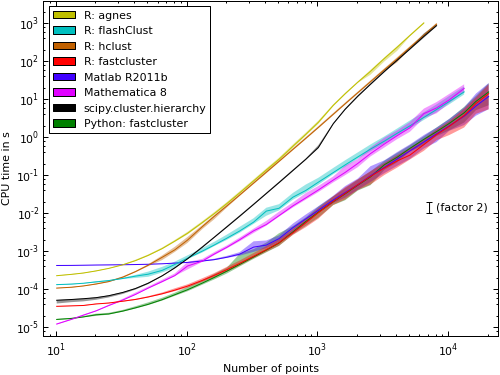
\includegraphics[scale=0.7]{images/FastComplete-CH3}
\caption[Complete linkage clustering speed comparison between popular implementations.]{The colored bands show maximum and minimum time over a variety of data sets. The average is plotted as a solid line. The synthetic data sets are samples drawn in an iid. manner from various mixtures of Gaussian distributions in Euclidean space of various dimensions.
%The results were obtained on a PC with an Intel dual-core CPU T7500 with 2.2 GHz clock speed and 4GB of RAM. The operating system was Ubuntu 11.04 64-bit (Ubuntu 10.04 64-bit for Matlab R2010a). R version: 2.13.0, fastcluster version: 1.1.7, flashClust version: 1.01, Python version: 2.7.1, NumPy version 1.5.1, SciPy version: 0.8.0.
(reprinted from \protect\cite{FastClust})}
\label{fig:FastClustComparison}
\end{figure}

I quickly linked up fastcluster to ES2, replacing our naive binning implementation and was achieving impressive speed results. However, we are not enthusiastic about adding another dependency to ES2. For now it's a envisioned improvement for the next version of ES.

%Include excel picture of comparison!


\subsubsection*{Minimizing space usage}
%None of that matters if we can't decrease the space usage.
%Approach one, don't save a divergence matrix
%Here I could include some of my code.
While
%Approach two, bin in parallel.

\subsection*{Parallelization}
%Talk a little bit about the parallelization plans we have. Hybrid mp and mph
%and how it'll be the next step in the ES evolution
\subsubsection*{OpenMP approach} %WIKI EXACT OPERATION OF OPENMP!!!
The OpenMP API is a commonly used shared-memory parallelism approach designed for C, C++, and Fortran programs.
In Fortran the programmer adds comments (known as directives) to specify OpenMP behavior.
These directives implicitly or explicitly define, perhaps guide, the execution of multiple threads as parallel programs

An OpenMP enriched program begins as a single thread of execution.
Whenever a thread encounters a parallel construct the thread creates a team of sub-threads, generates a set of tasks, and then declares itself master of the team.
Only the master thread resumes execution beyond the end of the parallel construct.
The program can specify any number of parallel constructs.

All threads have access to the same memory so they can retrieve variables, this is called a shared-memory model.
Also, each thread can specify private memory unreachable to other threads.
We use shared and private clause keywords to identify the respective paradigm.
%HERE LING REFERENCES AN ARTICLE

\subsubsection*{Tests}
%Outline best results from Ling's tests

%NEW CHAPTER FOR SHOWING COMPARISONS BETWEEN THE TWO
\gobbletocpage
\chapter{Systemic Testing of Available Bacteria Speciation Models}
\restoretocpage

\begin{shadequote}
I wanna make sure you're ready, brother. Here it is: Show me the money. Oh-ho-ho! SHOW! ME! THE! MONEY! A-ha-ha! Jerry, doesn't it make you feel good just to say that! Say it with me one time, Jerry. \par\emph{Rod Tidwell}
\end{shadequote}


\section{Methods}
Most methods used were based on a previous study, with few modifications~\cite{carlo}.
Our main goals were to test ES2's accuracy for small input sizes, large input sizes, and show ES2's speed improvements over ES1.
This involves many \emph{in silico} or computer generated dataset tests and a test of ES2 on previous \emph{Bacillus} data samples from Death Valley.

To test accuracy of different algorithms we utilized an established pipeline~\cite{carlo}, (see Figure~\ref{fig:ComparisonFlow}) which involves generating sequences, and a corresponding demarcation answer key in a standard format.
The generated sequences are then passed through all the demarcators, including a random demarcator (used as a control), producing clustering output in the established standard format.
We then use a metric to compare each resulting output to the corresponding answer key that gives a quantification for accuracy. Figure~\ref{fig:ComparisonFlow} on page \pageref{fig:ComparisonFlow} clearly shows the workflow for this pipeline.

Speed tests were done using the python time package to clock starting and finishing times of each algorithm several times, finding the mean running time on various datasets~\cite{carlo}.

\begin{figure}[h!]
\centering
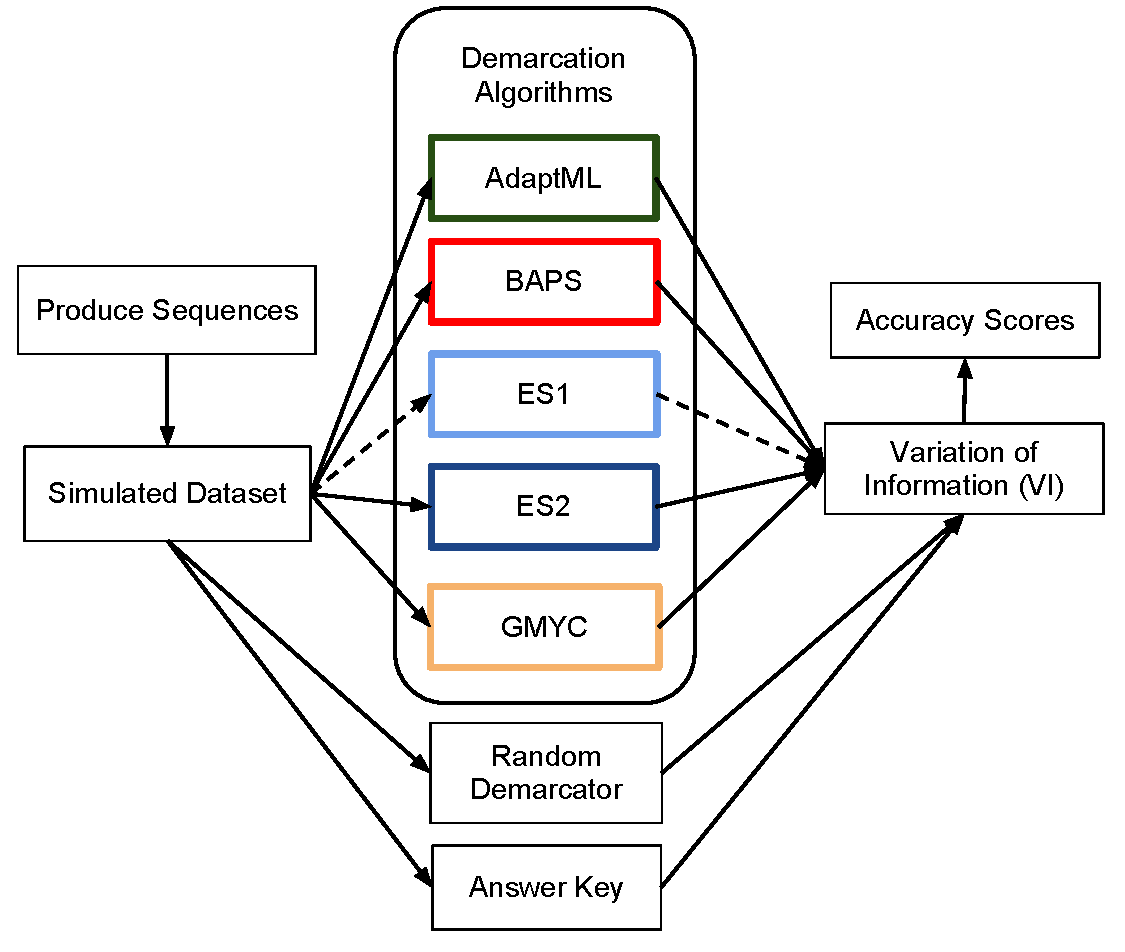
\includegraphics[scale=0.75]{images/DemarcationComparisonsFlow-CH4}
\caption[Demarcation comparison flow diagram.]{A flow diagram for the running of demarcation accuracy comparisons. The produce sequences makes simulated datasets that are used as inputs for various demarcation algorithms, the random demarcator, and answer key generation. Answer keys are generated directly from the knowledge involved in producing the sequences i.e., we know \emph{a priori} which strains belong in an ecotype and how many total ecotypes there are. All the resulting output is compared against the answer key with the Variation of Information (VI) metric to determine accuracy. The dotted line is present because ES1 is not run on the larger datasets.}
\label{fig:ComparisonFlow}
\end{figure}

\subsection*{Other demarcation algorithms}
As a rite of passage, we compare ES against other available demarcation algorithms~\cite{carlo}.
Previously, ES was demonstrated to be the most accurate, yet slowest demarcator.
ES2 aims to be just as accurate as ES but a lot faster, enabling larger input size functionality.
However, there are other demarcators currently available that utilize a variety of clustering models.

\subsubsection*{GMYC~\cite{barraclough2009inferring}}
The GMYC algorithm assumes a Yule model of speciation followed by a neutral coalescent model within species, where drift is the only process yielding coalescence.
It was originally designed to delineate species from sequences for sexually reproducing organisms such as insects, but later was shown to be applicable to asexually reproducing organisms.
GMYC needs only an ultrametric phylogentic tree to demarcate strains.
It is available as a part of the SPLITS package installed and imported onto any local R environment on Mac, Linux, and Windows.

\subsubsection*{BAPS~\cite{corander2007bayesian}}
The Bayesian Analysis of Population Structure (BAPS) application refines existing Bayesian approaches to determine the structure of populations from genetic data.
It assumes a partition-based mixture model and performs classification using a variant of the Metropolis-Hasting algorithm to identify clusters of sequences, with no explicit model of purging diversity within clusters.
Although, the algorithm can take into account recombination within and between populations.

BAPS has Windows, Linux and Mac versions with GUIs and a command line interface designed for batch processing; however it does not function in the Mac platform.

\subsubsection*{AdaptML~\cite{hunt2008resource}}
AdaptML places strains into ecotypes based on the assumption that the origin of each ecotype is driven by a change in habitat preferences.
Unlike the cohesion-based algorithms, it only requires a phylogentic tree and data specifying habitat isolation measurements for each strain.
The algorithm assumes a hidden Markov model for the evolution of habitat association and maximizes the likelihood of associations of the strains observed on the tree.

AdaptML runs on any operating system with a  version of Python installed. There is also a web app version of the algorithm where one can upload the data set and have AdaptML demarcations emailed.

\subsubsection*{Random demarcation}
I developed a random demarcator to serve as a control.
In it I pick a random number between one and the number of samples for $npop$ (we also experimented with variations of $npop$ choices, including using the correct $npop$). 
Then I randomly distribute the generated sequences throughout $npop$ ecotypes using the broken-stick model, and finally write a demarcation output file (see Figure~\ref{code:RandomDemarcating} on page~\pageref{code:RandomDemarcating}).

%Previous figure of code
%\begin{figure}[h!]
%\centering
%\noindent\code{Random Demarcation}{code/random_formatted.py}
%\caption[Python code showing a random demarcator.]{A description with more to be added soon, code needs to be cleaned up.}
%\label{code:RandomDemarcating}
%\end{figure}

\begin{figure}[h!]
\begin{algorithm}[H]
 \SetAlgoLined
% \KwData{c1 is a cluster of sequences, c2 is another cluster of sequences, seq-dist is a function that takes two sequences and returns the distance between them}
% \KwResult{the distance between two clusters}
\SetKwInOut{Input}{input}\SetKwInOut{Output}{output}

\Input{$sequences$ to be demarcated}
\Output{random demarcation based on broken stick distribution}
\BlankLine
 $randomNpop \gets $chooseNpop$(sequences)$\\
 $ecotypeDistribution \gets $[$|sequences|$]\\
 \While{$|ecotypeDistribution| \neq randomNpop$} {
 shuffle$(ecotypeDistribution$)\\
 $chosenEcotype \gets $pop$(ecotypeDistribution)$\\
 \If {$chosenEcotype \neq 1$} {
 $newEcotype1 \gets $random int between 1 and $(chosenEcotype - 1)$\\
 $newEcotype2 \gets chosenEcotype - newEcotype1$\\
 add $newEcotype1$ and $newEcotype2$ to $ecotypeDistribution$\\
 }
 }
 $ecotypes \gets \emptyset$\\
 shuffle$(sequences)$\\
 \For{$n \in ecotypeDistribution$} {
 add [$n$ popped individuals from $sequences$] to $ecotypes$\\
 }
 Write $ecotypes$ to output demarcation file\\
\end{algorithm}
\caption[Pseudocode showing a random demarcator.]{Pseudocode for the random demarcation algorithm. First a function is called to choose $npop$ (a separate function so we can easily modify how we choose $npop$ for variations of the algorithm). Then we form an ecotype distribution structure that has an integer entry per ecotype representing the number of sequences in the ecotype. We randomly choose an ecotype to split into two separate ecotypes (known as the broken-stick algorithm) until we have the same number of ecotypes as chosen $npop$. Finally, we distribute sequences according to the established ecotype distribution, and write the output file.}
\label{code:RandomDemarcating}
\end{figure}


\subsection*{Generation of sequences for analysis}
In order to compare the accuracy of several demarcation programs, the true parameters of the test data must be known.
The problem can be summarized as generating a history for a monophyletic group of $x$ organisms.
Clade history was based on an ecotype formation rate ($\Omega$), the rate of periodic selection ($\sigma$), and the number of ecotypes (\emph{npop}) within the sample.
We used the Ecotype Simulation algorithm to generate each organism's sequence and ecotype affiliation.
Habitats were indicated by either an ``A'' or ``B'', and favored habitat switches with each ecotype formation.
We generated datasets with differing numbers of simulated sequences, and based them on three values each of $\Omega$ and $\sigma$.
The middle values of $\Omega$ and $\sigma$ were 0.19 and 1.1 respectively, based on prior ES simulation of \emph{Bacillus} in a Death Valley canyon.
Lower and upper values represented a difference of a factor of 10 of the \emph{Bacillus} values.
$Npop$ values were chosen based on the specific run's input size.
We generally tried to choose $npop$ values of 10, 30, and 40 percent regarding input size.

\subsubsection*{Preparing the input}
PhyML~\cite{guindon2010new}, a maximum likelihood tree construction algorithm, was used to build a phylogenetic tree from generated sequences.
The tree was converted into an ultrametric chronogram using Sanderson's nonparametric rate smoothing algorithm, which is included in the APE package.
This ultrametric tree was used as input for GMYC.

AdaptML requires the habitat from which each strain was isolated.
In previous studies we designed a specialization metric for designating habitats, however we found a specific unit of this metric that worked best~\cite{carlo}.
Thus, we will stick to using the best parameter of habitat specialization for AdaptML analysis.

FASTA sequences were converted into XLS format for compatibility with the BAPS package.

\subsection*{Variation of Information Metric}
The Variation of Information (VI) metric~\cite{meilua2003comparing} was used as a criterion for comparing two partitions of the same data set, to determine the closeness of each algorithm's ecotype demarcations to the canonical demarcations generated \emph{in silico}.
The Variation of Information between two clusterings C and C' is given by$$VI(C, C') = H(C) + H(C') - 2I(C, C')$$where H(C) is the entropy of a random variable associated with a sequence being in a cluster C and I(C,C') is the mutual information of the two associated variables.

\subsection*{ES2 on smaller datasets}
I ran the new and improved ES2 algorithm on generated datasets for parameters clearly defined in previous studies~\cite{carlo}.
All sample datasets included fifty sequences, and repeated ten times to find the mean Variation of Information score (see Figure~\ref{fig:ESvES2}).
Notice how closely the two lines are on the horizontal axis.

On a few specific values we ran ES1 and ES2 through one hundred repetitions to find more robust VI scores.

\subsubsection*{Bacillus sequences}
\emph{Bacillus} strains were isolated from Radio Facility Wash, a west-running canyon in Death Valley, consisting of a habitats with three levels of solar exposure, including the canyon's sunny south-facing slope, the shadier and cooler north-facing slope, and the arroyo at the bottom~\cite{connor2010ecology}.
Solar exposure habitats served as the only ecological dimension used for environmental input into AdaptML.
Sequences were processed as previously reported~\cite{carlo}.
Again we used PhyML to produce a maximum likelihood tree.

\subsection*{All demarcation programs on large datasets}
We ran all demarcation programs, and a random demarcator on generated datasets of 50 (see Figure~\ref{fig:All50} on page~\pageref{fig:All50}), 100 (see Figure~\ref{fig:All100} on page~\pageref{fig:All100}), and 200 (see Figure~\ref{fig:All200} on page~\pageref{fig:All200}) sequences.
Parameters were once again adopted from previous studies.
The exception being a choice of $npop$ which, was three of 10, 20, 30, 40, 50.
We tried to pick $npop$ values that would hit the sweet spot of demarcation in addition to an upper and lower bound (i.e., regarding VI accuracy scores).

\subsection*{Running Time Tests}
We tested the running time of each algorithm on a 2.66GHz Intel Core 2 Duo processor with 4GB of RAM running Windows 7.
We present the mean run times that each algorithm required to analyze synthetic data sets constructed using the parameter values estimated previously for \emph{Bacillus}, with various input sizes, and at least 5 repetitions.

\section{Results and Discussion}

%Proof of concept for a figure!
%\begin{figure}[h!]
%  \caption[Demarcation comparison table for small inputs (nu = 50).]{A comparison table of all demarcation algorithms run with differing sigma, omega, and npop values on input sizes of 50 sequences. Parameter combinations in which ES2 outperformed ES1 are circled in red. [I probably won't put in the full table, but parts of it and leave the big one for the appendix]}
%  \centering
%    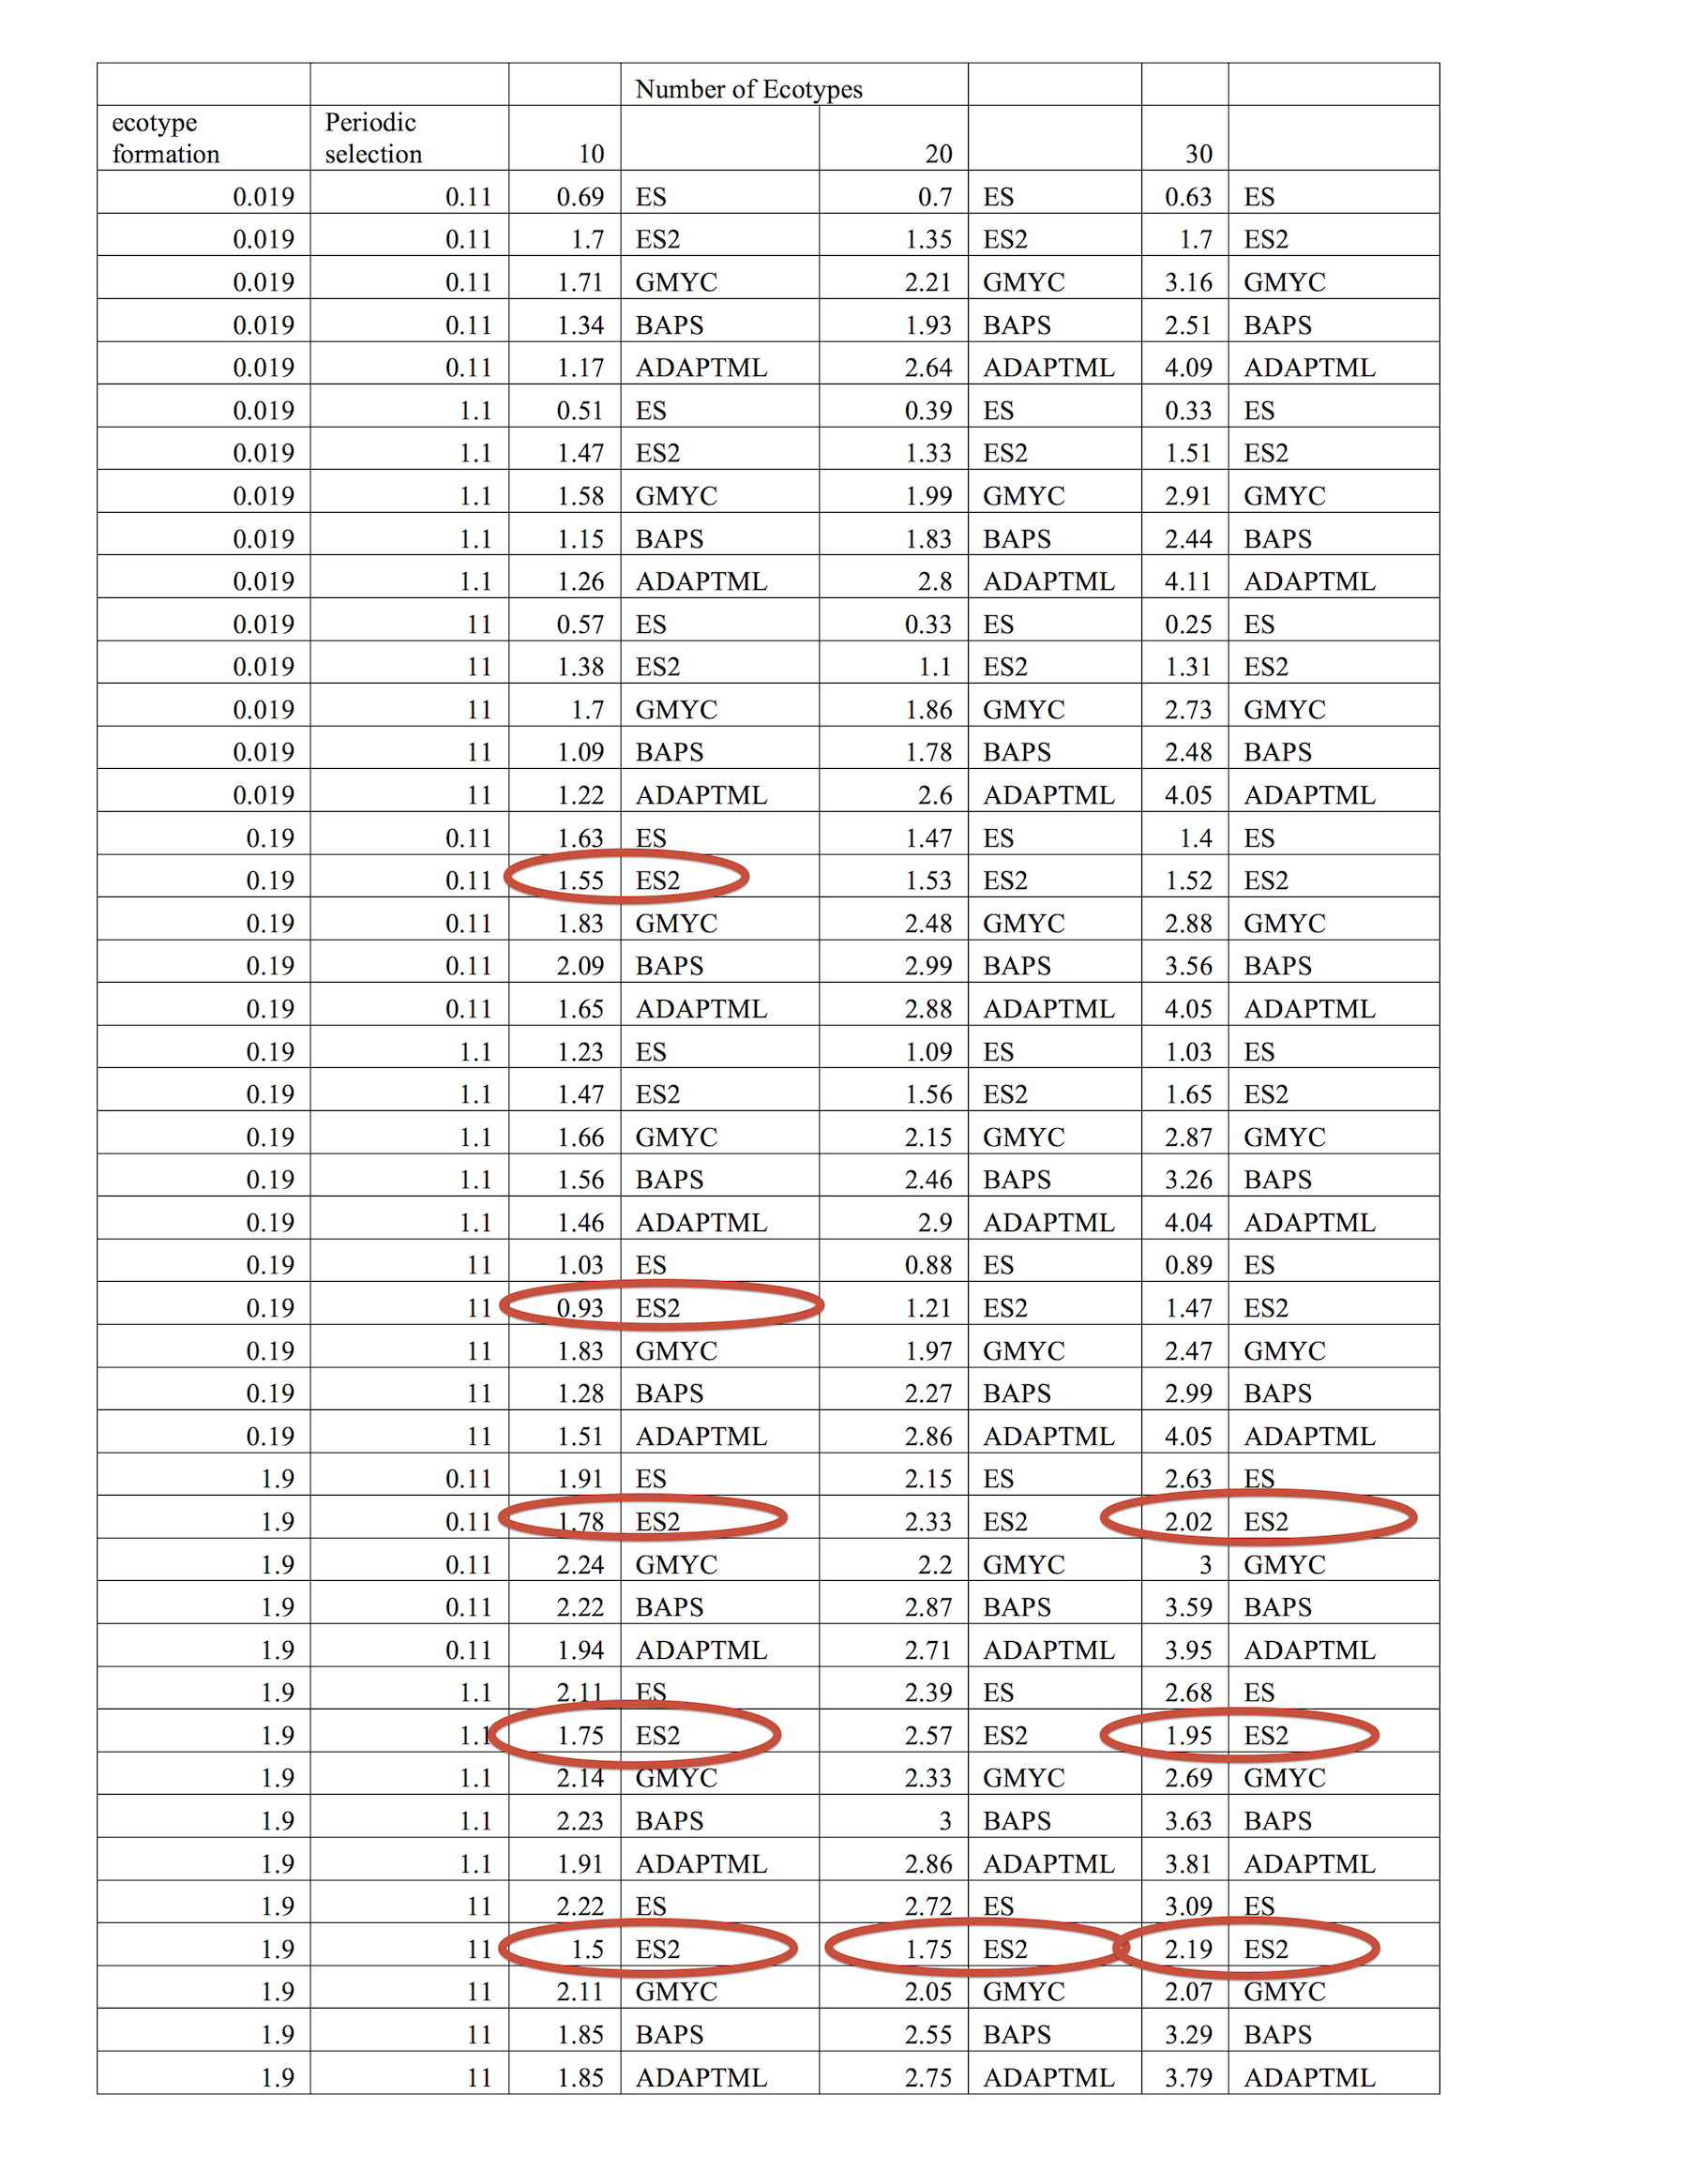
\includegraphics{images/ComparisonTable1.png}
%    \label{fig:ComparisonSmall}
%\end{figure}

\subsection*{Analysis of in silico-generated sequences}
The majority of my work was putting together a database of in silico generated sequences demarcation runs.
A lot of the code I used to run tests was legacy code from past lab members.
I had to update many dependency packages, and modify certain portions to work on various computer platforms.
BAPS does not run on with batch mode on Macintosh.
GMYC worked half of the time, and other times there was an error based on tree generation.
Some analysis does not include GMYC due to this unresolved issue.

\subsubsection*{ES2 on smaller datasets}
Our first experiment was to run Ecotype Simulation (ES) and Ecotype Simulation 2 (ES2) on smaller datasets (i.e., $nu = 50$) and checking accuracy (VI) scores (see Figure~\ref{fig:ESvES2}).

%Nested npop, omega, sigma
\begin{figure}[h!]
  \centering
    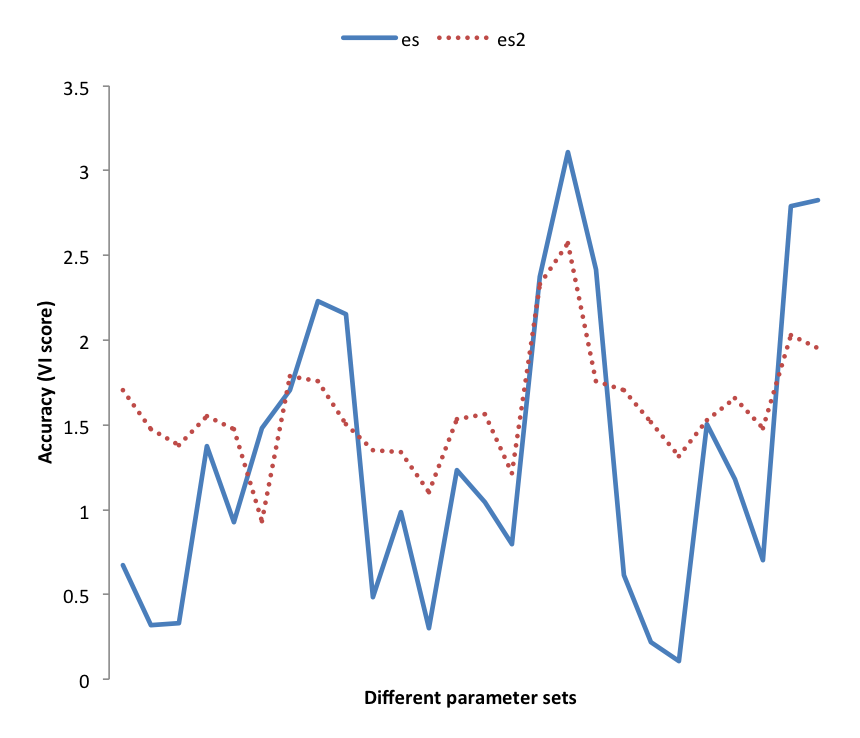
\includegraphics[scale=0.75]{images/ResultGraphs/ResultGraphs-4}
      \caption[ES vs ES2 accuracy visualization on $nu = 50$.]{Across 27 parameter set combinations I exhaustively test ES (solid line) and ES2 (dotted line) on $npop$ values of 10, 20, and 30, $\Omega$ values of 0.019, 0.19, and 1.9, $\sigma$ values of 0.11, 1.1, and 11, for nu of 50 sequences. On the $y$-axis we have VI scores, where values closer to 0 represent more accurate demarcation runs.}
    \label{fig:ESvES2}
\end{figure}

Notice how closely the two lines are.
ES (solid line) is generally lower (i.e., more accurate), however there are dramatic peaks and valleys of performance.
In contrast to ES2 (dotted) which overall quite accurate with few valleys and peaks.

\begin{table}
    \begin{tabular}{l|cc}
    ~                  & Ecotype Simulation & Ecotype Simulation 2 \\ \hline
    Average            & 1.30414053         & 1.596300918          \\
    Standard Deviation & 0.877454163        & 0.343838045          \\
    \end{tabular}
    \caption[ES versus ES2 statistics.]{Statistics on the ES vs ES2 run with 10 reps on a dataset of $nu=50$.}
    \label{tab:ESvES2mean}
\end{table}

This trend is represented in Table~\ref{tab:ESvES2mean} on page~\pageref{tab:ESvES2mean}, by ES2's lower standard deviation than ES1.
However, ES still has a lower mean VI score, but not by much.

From these tests, we feel fairly confident in ES2's accuracy.
Across various parameters ES2 looks to be more consistent than even ES1, even though ES1 demarcation matches more closely the answer demarcation more often.
On small datasets speed is not too much of an issue, but if you want to run a lot of small datasets, then we advise using ES2.

\subsubsection*{All demarcation programs on large datasets}
Once we run Ecotype Simulation on datasets of 50 sequences are larger time becomes a significant issue.

For this reason we developed ES2 to run on datasets with more than 50 individuals.
However from past studies we found ES to be the most accurate demarcating program, and we would expect this level of accuracy from ES2 on larger datasets.

%\begin{figure}[h!]
%  \centering
%    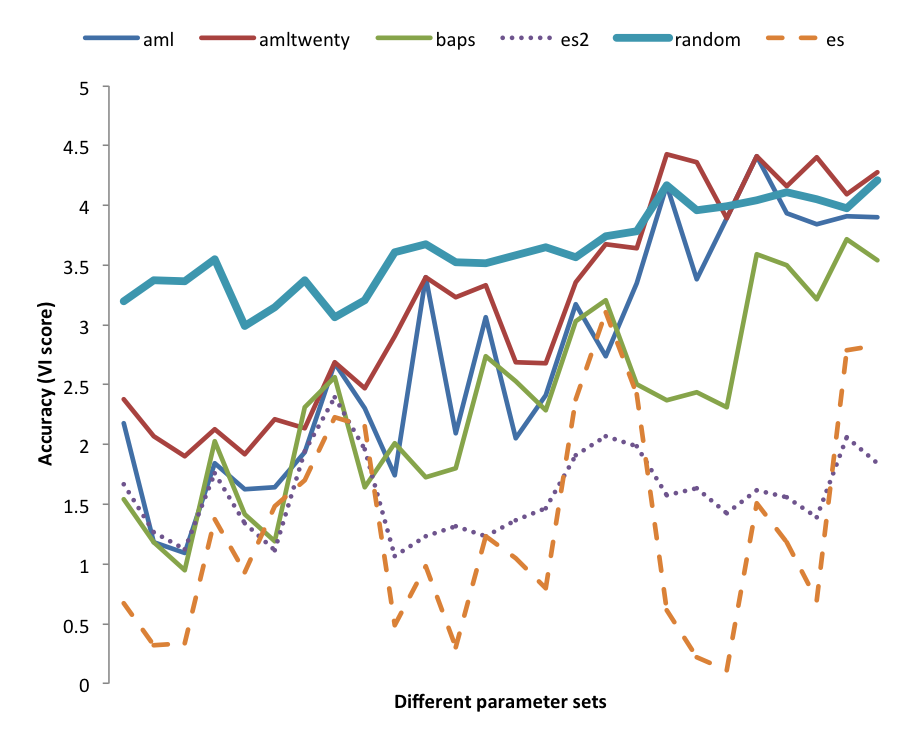
\includegraphics[scale=0.75]{images/ResultGraphs/ResultGraphs-3}
%      \caption[All demarcation graphical accuracy visualization on $nu = 50$.]{Across 27 parameter set combinations I exhaustively test all demarcation programs on $npop$ values of 10, 20, and 30, $\Omega$ values of 0.019, 0.19, and 1.9, $\sigma$ values of 0.11, 1.1, and 11, for nu of 50 sequences. Random demarcation is represented by the solid line. On the $y$-axis we have VI scores, where values closer to 0 represent more accurate demarcation runs.}
%    \label{fig:All50}
%\end{figure}
%
%\begin{table}
%    \begin{tabular}{l|ccccc}
%    ~                  & AdaptML     & AdaptML$^\ast$    & Baps        & Ecotype Simulation 2 & Random      \\ \hline
%    Average            & 2.767371639 & 3.185623443 & 2.359650359 & 1.589546505          & 3.631545086 \\
%    Standard Deviation & 0.971373851 & 0.868775294 & 0.783228066 & 0.34336826           & 0.34949857  \\
%    \end{tabular}
%    \caption[Statistics on all demarcators on $nu=50$.]{Statistics on all demarcators run with 5 reps on a dataset of $nu=50$.}
%        \label{tab:50Allmean}
%\end{table}

\begin{figure}[h!]
  \centering
    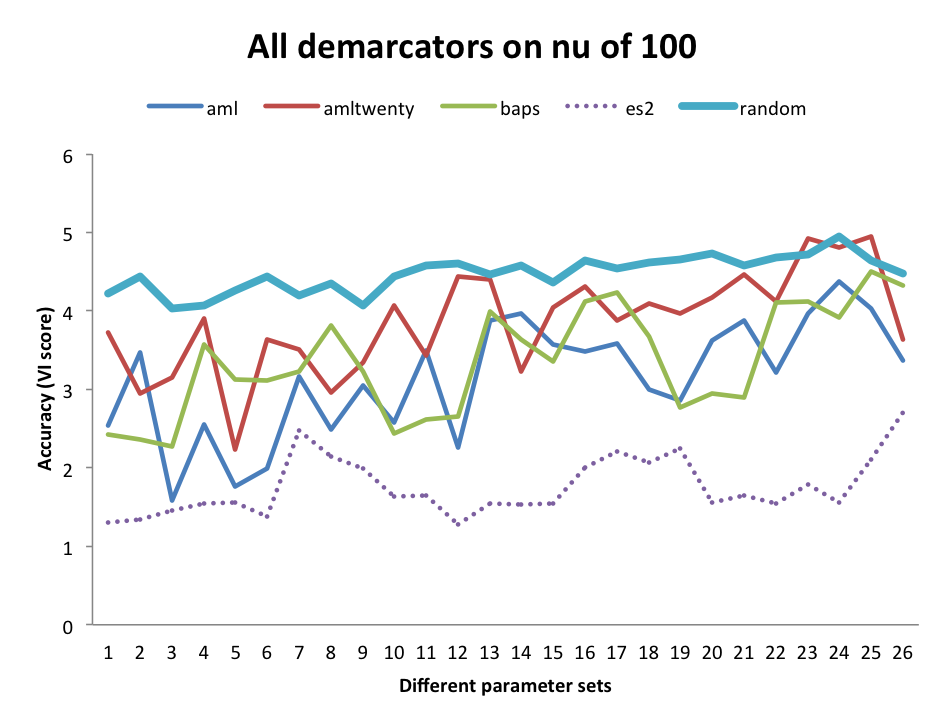
\includegraphics[scale=0.75]{images/ResultGraphs/ResultGraphs-2}
      \caption[All demarcation graphical accuracy visualization on $nu = 100$.]{Across 27 parameter set combinations I exhaustively test all demarcation programs on $npop$ values of 30, 40, and 50, $\Omega$ values of 0.019, 0.19, and 1.9, $\sigma$ values of 0.11, 1.1, and 11, for nu of 100 sequences. Random demarcation is represented by the solid line. On the $y$-axis we have VI scores, where values closer to 0 represent more accurate demarcation runs.}
    \label{fig:All100}
\end{figure}

Figure~\ref{fig:All100} on page~\pageref{fig:All100} shows accuracy scores for all demarcating programs on a variety of parameters (bacillus values with .1x and 10x and $npop$ values of 30, 40, 50) on sample size of 100 individuals.
Notice that overall ES2 (dotted line) was the lowest (i.e., most accurate), that means ES2's demarcation output matched most closely to the answer key demarcations.

This fact is highlighted by the lowest average VI score shown in Table~\ref{tab:100Allmean}, of 1.76.
Also, notice that once again ES2 has the lowest standard deviation, meaning that it was the most consistent, except of course for the random demarcation, which was consistently terrible accuracy wise (as we would expect).
ES2 was followed by AdaptML(3.14), BAPS (3.36), and Random (4.47).
With less habitat specialization AdaptML lost accuracy.

ES2 appeared to be slightly more accurate with higher $npop$ values; the gap between it and other demarcators increased.
Higher rates of $\Omega$ (rate of ecotype formation) resulted in slight increases in ES2 VI scores.
It appears that changes in $\sigma$ (rate of periodic selection) did not affect the accuracy of each algorithm as much as modifying $\Omega$.
$Npop$ appears to have had the greatest effect on the accuracy of all the demarcation programs, least of all ES2.
Losing accuracy with greater values of $npop$ was a trend that continued with larger datasets (see supplementary figures in appendix).

\begin{table}[h!]
    \begin{tabular}{l|ccccc}
    ~                  & AdaptML     & AdaptML$^\ast$     & BAPS        & Ecotype Simulation 2 & Random      \\ \hline
    Average            & 3.142555041 & 3.860006018 & 3.363530792 & 1.762829323          & 4.475184564 \\
    Standard Deviation & 0.727870506 & 0.639625177 & 0.67100242  & 0.370748481          & 0.225368714 \\
    \end{tabular}
    \caption[Statistics on all demarcators on $nu=100$.]{Statistics on all demarcators run with 5 reps on a dataset of $nu=100$. ($^\ast$) Represents AdaptML ran with a habitat specialization value of 20.}
        \label{tab:100Allmean}
\end{table}

Tests regarding large datasets are ongoing.
In the appendix you can find additional graphs with all demarcators for nu of 50 and 200 along with corresponding tables showing mean and standard deviation values.
As of yet these tests were done on only 5 repetitions.
We would like repetitions in the hundreds.

%
%\begin{figure}[h!]
%  \centering
%    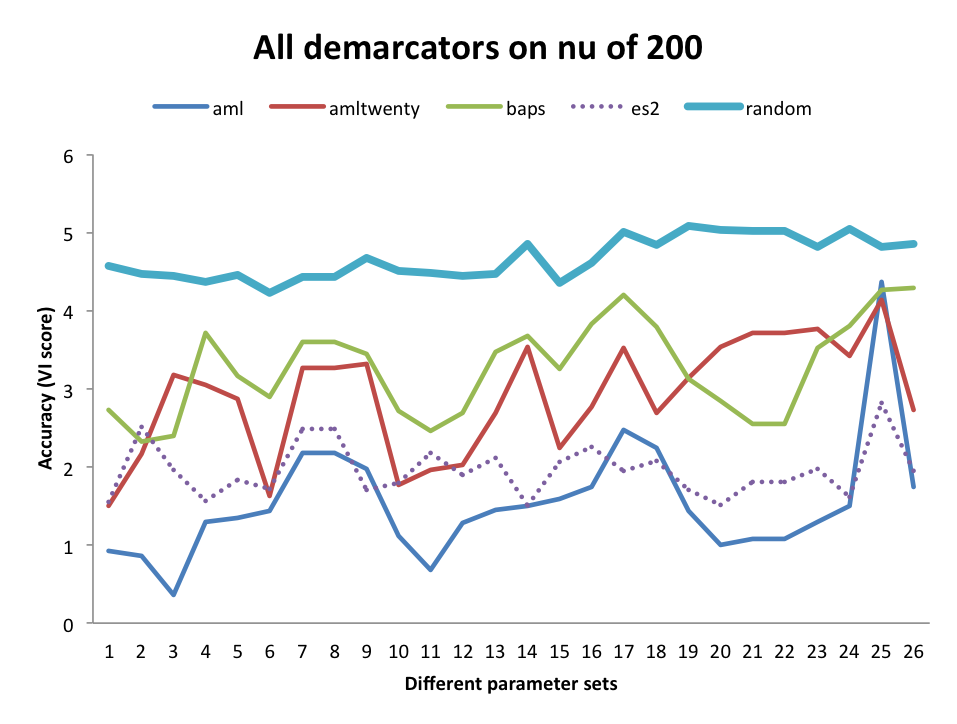
\includegraphics[scale=0.75]{images/ResultGraphs/ResultGraphs-1}
%      \caption[All demarcation graphical accuracy visualization on $nu = 200$.]{Across 27 parameter set combinations I exhaustively test all demarcation programs on $npop$ values of 30, 40, and 50, $\Omega$ values of 0.019, 0.19, and 1.9, $\sigma$ values of 0.11, 1.1, and 11, for nu of 200 sequences. Random demarcation is represented by the solid line. On the $y$-axis we have VI scores, where values closer to 0 represent more accurate demarcation runs.}
%    \label{fig:All200}
%\end{figure}
%
%\begin{table}
%    \begin{tabular}{l|ccccc}
%    ~                  & AdaptML     & AdaptML$^\ast$     & BAPS        & Ecotype Simulation 2 & Random      \\ \hline
%    Average            & 1.543424394 & 2.908133924 & 3.265003881 & 1.955714164          & 4.667531001 \\
%    Standard Deviation & 0.748104722 & 0.713876097 & 0.59283446  & 0.33348659           & 0.258112685 \\
%    \end{tabular}
%    \caption[Statistics on all demarcators on $nu=200$.]{Statistics on all demarcators run with 5 reps on a dataset of $nu=50$.}
%        \label{tab:200Allmean}
%\end{table}

\subsection*{\emph{Bacillus} sequences}
I ran ES2 on \emph{Bacillus} sequences from previous studies.
The results were consistent with previous demarcation runs (see Figure~\ref{fig:Bacillus} on page~\pageref{fig:Bacillus}).

\begin{figure}[h!]
  \centering
    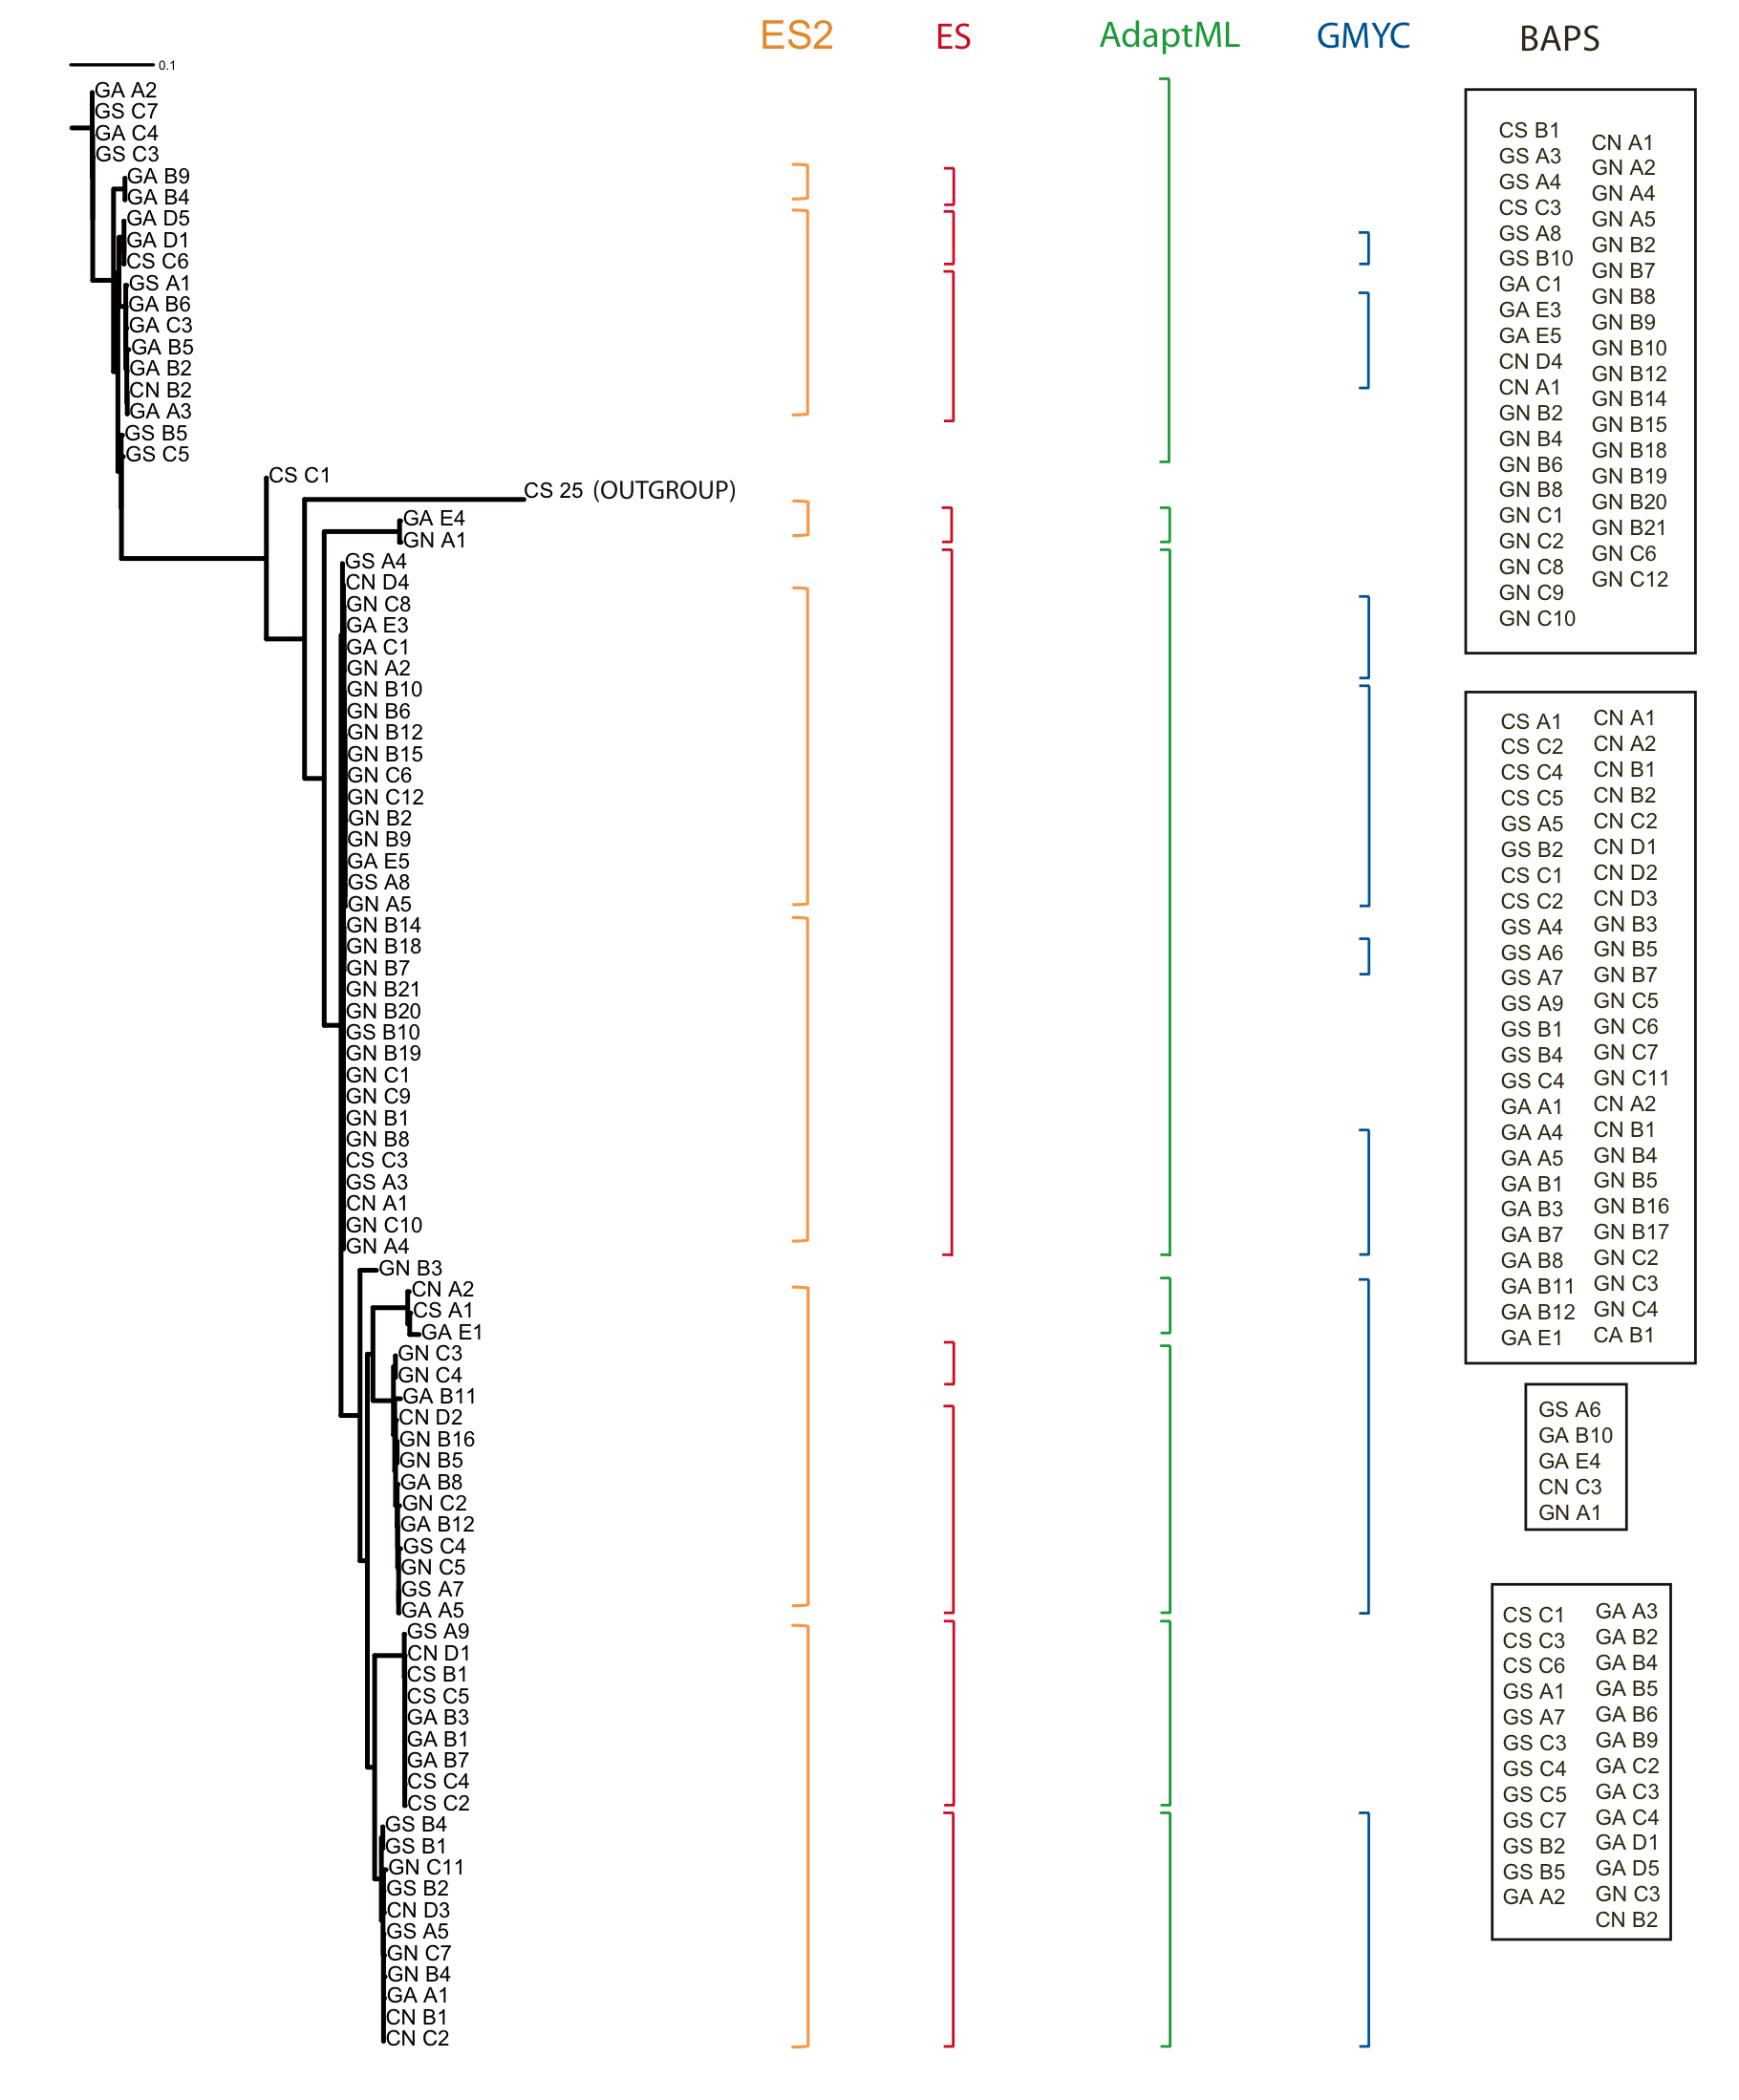
\includegraphics[scale=0.7]{images/Bacillus-CH4}
      \caption[Demarcation programs run on previous \emph{Bacillus} sequences.]{Demarcation programs run on previous \emph{Bacillus} sequences. [ADD OTHER DEMARCATORS]}
    \label{fig:Bacillus}
\end{figure}

\subsection*{Running time}
We compared the running times of the demarcation algorithms on synthetic data sets of different sizes, and found that AdaptML, GMYC, and BAPS performed demarcations much more quickly then ES2 (see Figure~\ref{fig:WindowsSpeed}).
AdaptML, GMYC, and BAPS all completed demarcations on the order of a few seconds, even for data sets in the hundreds whereas ES required on the order of tens of minutes for the same inputs.
GMYC was the fastest algorithm, taking no more than one second on average.
AdaptML followed, and BAPS was the slowest of the three faster algorithms.

\begin{figure}[h!]
  \centering
    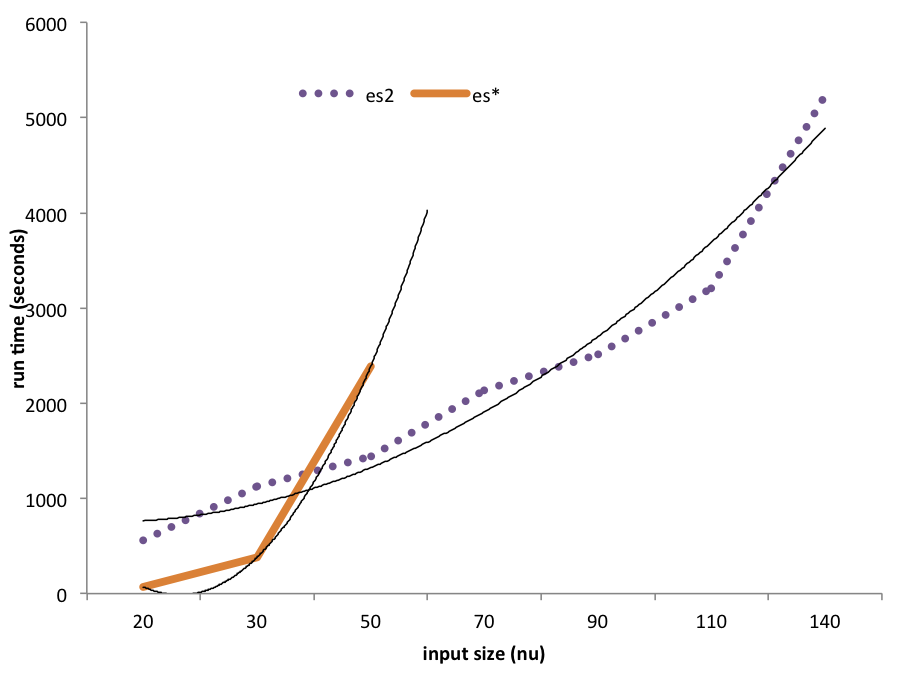
\includegraphics[scale=0.7]{images/SpeedWindows-CH4}
      \caption[Demarcation run time test on Windows.]{Comparison of demarcation runtimes on a Windows. The dotted line represents ES2's runtime. Most demarcators run completely within seconds.}
    \label{fig:WindowsSpeed}
\end{figure}

Since the BAPS's batch processing feature was not available for Mac I ran it on Windows.
However, I also ran ES2, GMYC, and AdaptML separately on my Mac and found that ES2 was significantly faster than when it was run on a Windows machine.

\subsubsection*{Automatic demarcation}
We found that automatic demarcation was taking approximately 90\% of the ES2 run time.

\section{Chapter Summary}
In this chapter I discussed the motivation and thought process behind our experiments.
I gave a survey of other available demarcation programs (GMYC, BAPS, AdaptML) and our control random demarcator, how we generated sample datasets, and described the metric used to compare the various outputs (Variation of Information metric).

First we wanted to show that ES1 and ES2 achieve similar levels of accuracy.
Thus we ran ES1 and ES2 on data sets with 50 individuals for 10 repetitions.
ES2 achieved comparable accuracy, and had a lower standard deviation.

Next, we ran all the demarcator programs on various sized data sets.
ES2 maintained a high level of accuracy throughout a wide range of parameters (based on previous \emph{bacillus} values).

Traditionally we run all demarcators on \emph{Bacillus} sequences.
We found ES2 performed well.

Once again ES2 was the slowest demarcation algorithm.
However, it improved dramatically on ES1 running times.



\gobbletocpage
\chapter{Conclusion}
\restoretocpage

%\pagestyle{chapter}
\begin{shadequote}
Still thinking about a quote to finish it. \par--\emph{Diego Calderon}
\end{shadequote}

%Some kind of end of something quote. Maybe the famous last words of a book.
%He loved Big Brother  hahahaha

\section{Final remarks on ES}

%Re-iterate motivation and purpose of bacterial demarcations
Re-iterate motivation and purpose of bacterial demarcations


%Talk a little bit about the background and ES
Talk a little bit about the background and ES

%Talk a little bit about the improvements, resulting in ES2
Talk a little bit about the improvements, resulting in ES2

%Summarize ES2 vs ES and ES2 vs all results
Summarize ES2 vs ES and ES2 vs all results

%Concluding analaysis
Concluding analaysis
...and that is why ES is the best.

However, we should use a combination of approaches, each lending strengths to the other's weaknesses, adding robustness to microbial ecosystem analysis~\cite{bohannan2003new}

\section{For the future}
%Might not need this section, then again some repetition might be good?
Continue to work on ES.
Specific issues with a short description, speed, binning, space usage, demarcation.
Perhaps include small blurb of future wet lab plans?


\bibliography{references}
\addcontentsline{toc}{chapter}{Bibliography}
%Might not be needed toc is already 2 pages?
\addcontentsline{toc}{chapter}{Index}

%\include{glossary}
%\include{notat}
%\bibliographystyle{amsalpha} %The style you want to use for references.
%\bibliography{mr,refs} %The files containing all the articles and books you ever referenced.
\printindex %Make an index AUTOMATICALLY

\end{document}